\documentclass[10pt,twocolumn,letterpaper]{article}

\usepackage{cvpr}
\usepackage{times}
\usepackage{epsfig}
\usepackage{graphicx}
\usepackage{amsmath}
\usepackage{amssymb}

% Include other packages here, before hyperref.
\usepackage{tabularx} % in the preamble
\newcolumntype{Y}{>{\centering\arraybackslash}X}
\newcommand\VRule[1][\arrayrulewidth]{\vrule width #1}
\usepackage{array,booktabs,arydshln,xcolor} % for widening table line
\usepackage{amsthm,bm}
\usepackage{epstopdf}
\usepackage[flushleft]{threeparttable}
\usepackage{amsthm}
\usepackage{multirow}

\usepackage{float}
\usepackage{wrapfig}
\usepackage{subcaption}
\usepackage{capt-of}% or \usepackage{caption}
\usepackage{booktabs}
\usepackage{varwidth}
\usepackage{wrapfig}
\usepackage{makecell}

\usepackage{algpseudocode,algorithm,algorithmicx}
\newcommand*\DNA{\textsc{dna}}

\newcommand*\Let[2]{\State #1 $\gets$ #2}
\algrenewcommand\algorithmicrequire{\textbf{Precondition:}}
\algrenewcommand\algorithmicensure{\textbf{Postcondition:}}


\makeatletter
\def\BState{\State\hskip-\ALG@thistlm}
\makeatother

\usepackage{bm}

\usepackage[pagebackref=true,breaklinks=true,letterpaper=true,colorlinks,bookmarks=false]{hyperref}

%\cvprfinalcopy % *** Uncomment this line for the final submission

\def\cvprPaperID{****} % *** Enter the CVPR Paper ID here
\def\httilde{\mbox{\tt\raisebox{-.5ex}{\symbol{126}}}}

% Pages are numbered in submission mode, and unnumbered in camera-ready
%\ifcvprfinal\pagestyle{empty}\fi
%\setcounter{page}{4321}
\begin{document}

%%%%%%%%% TITLE
\title{Photographic Text-to-Image Synthesis \\ with a Hierarchically-nested Adversarial Network}

\author{First Author\\
Institution1\\
Institution1 address\\
{\tt\small firstauthor@i1.org}
% For a paper whose authors are all at the same institution,
% omit the following lines up until the closing ``}''.
% Additional authors and addresses can be added with ``\and'',
% just like the second author.
% To save space, use either the email address or home page, not both
\and
Second Author\\
Institution2\\
First line of institution2 address\\
{\tt\small secondauthor@i2.org}
}

\maketitle
%\thispagestyle{empty}

%%%%%%%%% ABSTRACT
\begin{abstract}
This paper presents a novel method to deal with the challenging task of generating images conditioned on semantic image descriptions. We propose an effective end-to-end single-stream network that can generate photographic high-resolution images. Our method leverages the deep representations of convolutional layers and introduces accompanying hierarchical-nested adversarial games inside the network hierarchy, which regularize intermediate representations and assist training to capture the complex image statistics. We present an extensile network architecture to cooperate with discriminators and push generated images to high resolutions. 
We adopt a multi-purpose adversarial training strategy at multiple nested side outputs to encourage more effective image-text alignment in order to guarantee the semantic consistency and image fidelity simultaneously. Furthermore, we introduce a new visual-semantic similarity measure to evaluate the semantic consistency of generated images.
With extensive experimental validation on three major datasets, our method significantly improves previous state of the arts on all datasets over different evaluation metrics. 
\end{abstract}


%%%%%%%%% BODY TEXT
\section{Introduction}
Photographic text-to-image synthesis is a significant problem in generative model research \cite{reed2016generative}, which aims to learn a translation from a semantic text embedding space to a complex RGB image space. This task requires the generated images to be \textit{semantically consistent}, i.e., the generated images not only preserve sketch concepts in descriptions but also fine-grained descriptive details in image pixels. 
However, insufficient methods are developed to successfully address this task due to its particular challenges. 

%It is a special case of generative learning tasks, which aim to map a low-dimensional embedding to a complex RGB image space. Differently, the embedding space of the former is induced by semantic descriptions. Therefore, this task requires the generated images to be \textit{semantically consistent}, i.e., the generated images not only preserve sketch concepts of descriptions but also fine-grained descriptive details in image pixels. 

\begin{figure}[t]
%	\begin{center}
	\centering
	\begin{subfigure}[t]{0.5\textwidth}
	%	\centering
		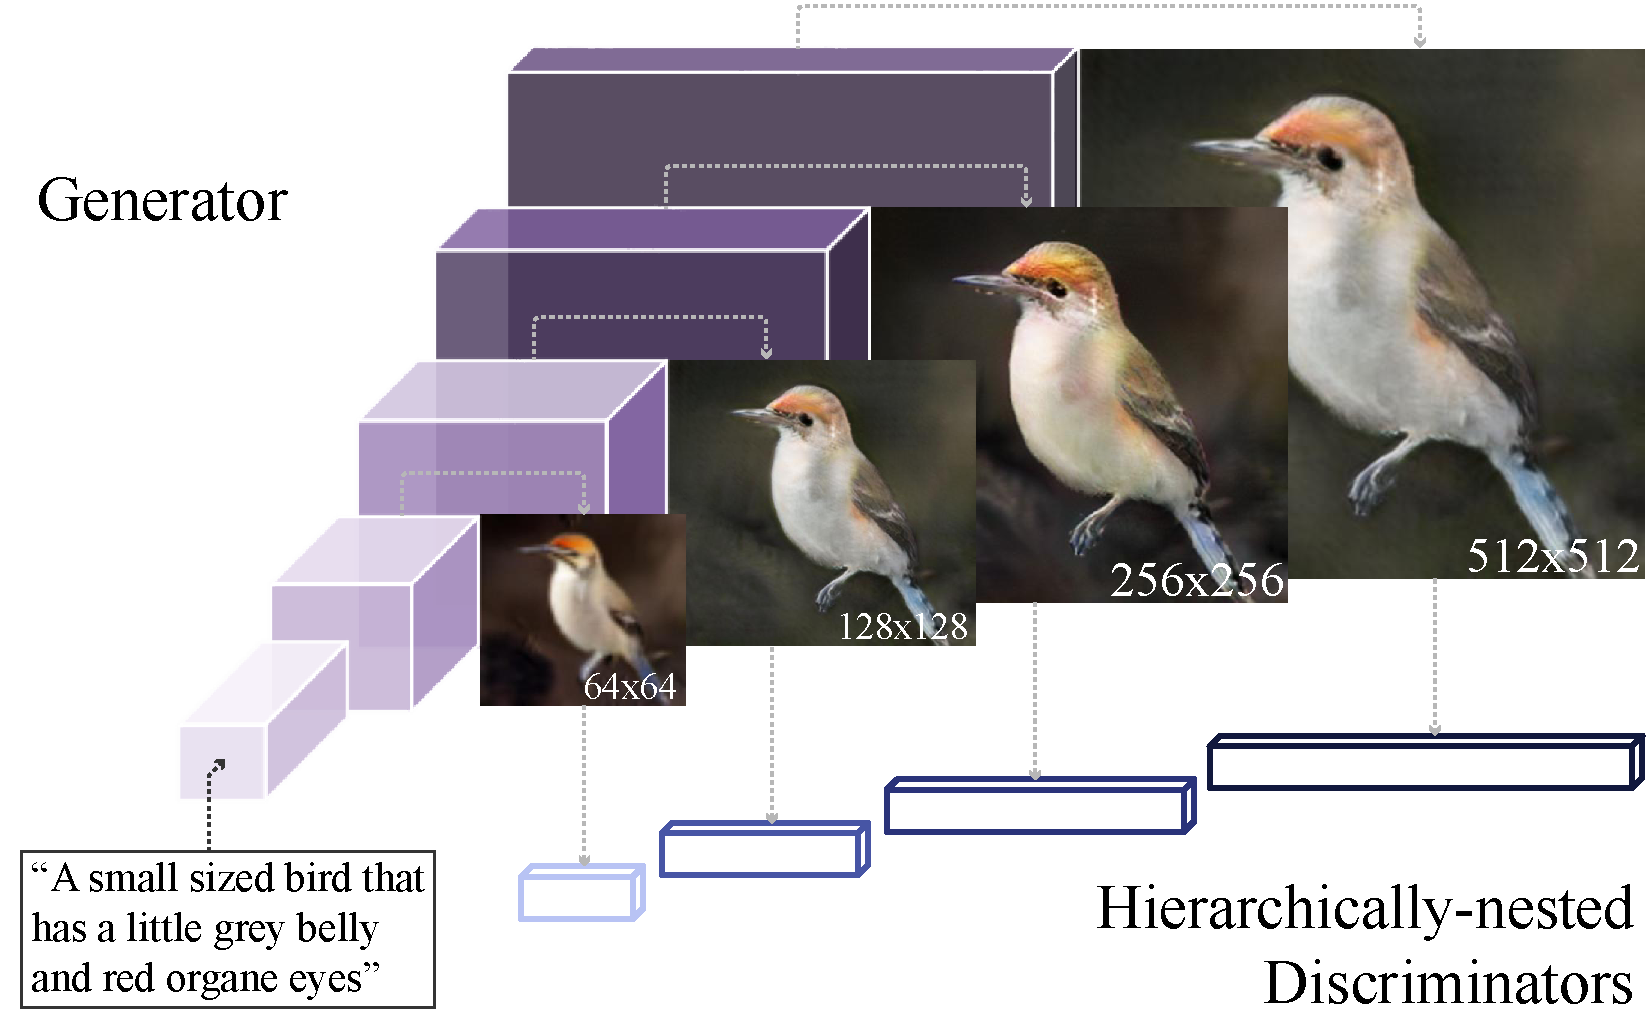
\includegraphics[width=0.95\textwidth]{figure/intro2.pdf}
	\end{subfigure} \\
\centering
	\begin{subfigure}[t]{0.5\textwidth}
	%	\centering
		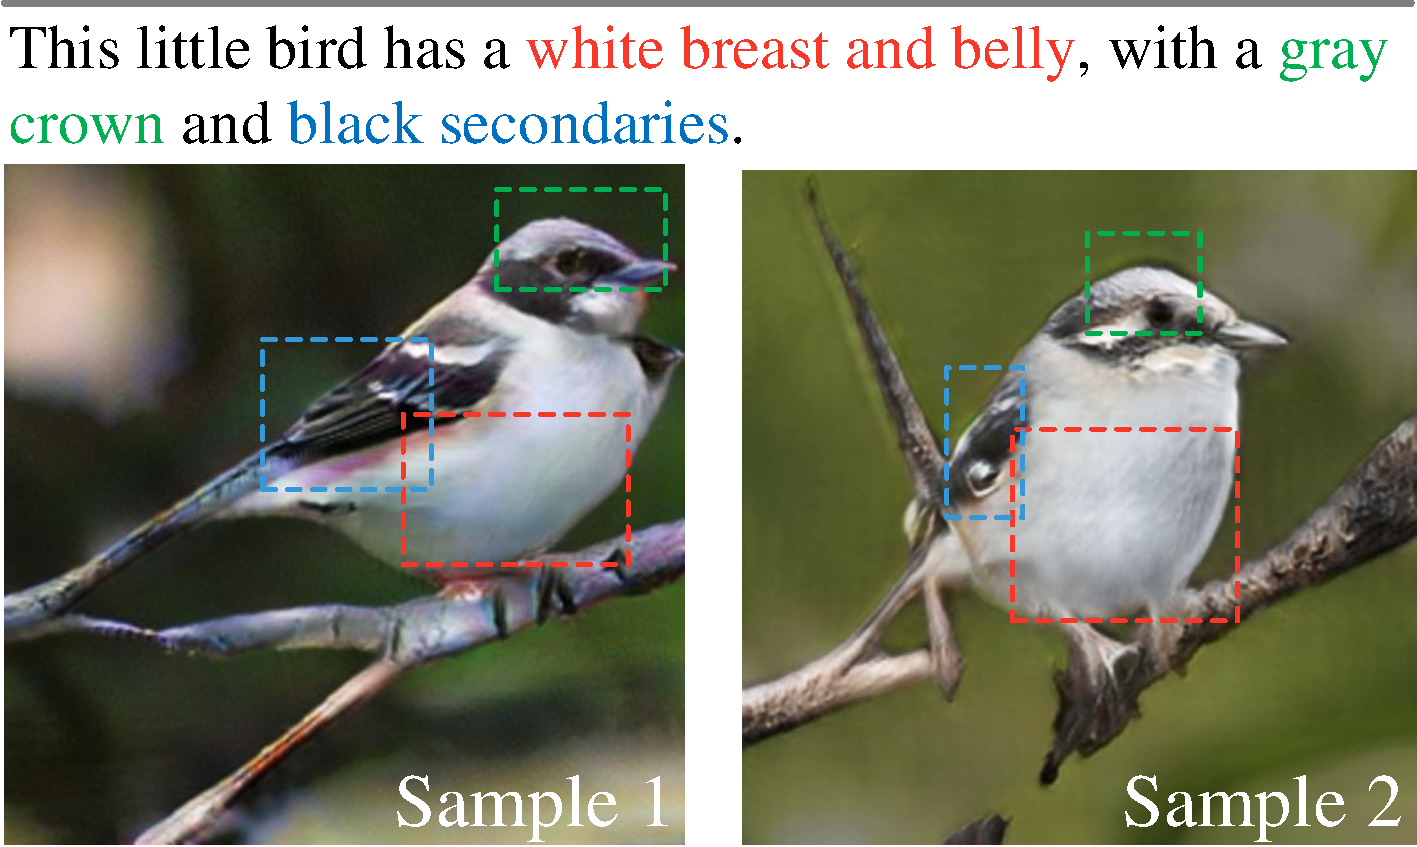
\includegraphics[width=0.95\textwidth,height=0.55\textwidth]{figure/single_view.pdf}
	\end{subfigure}
	\vspace{-.6cm}
	\caption{Top: Overview of our hierarchically-nested adversarial network. Bottom: Two fine-grained generated results. \label{fig:intro}} 	
	\vspace{-.8cm}
	%\end{center}
\end{figure}


%\begin{figure}[t]
%	\centering
%	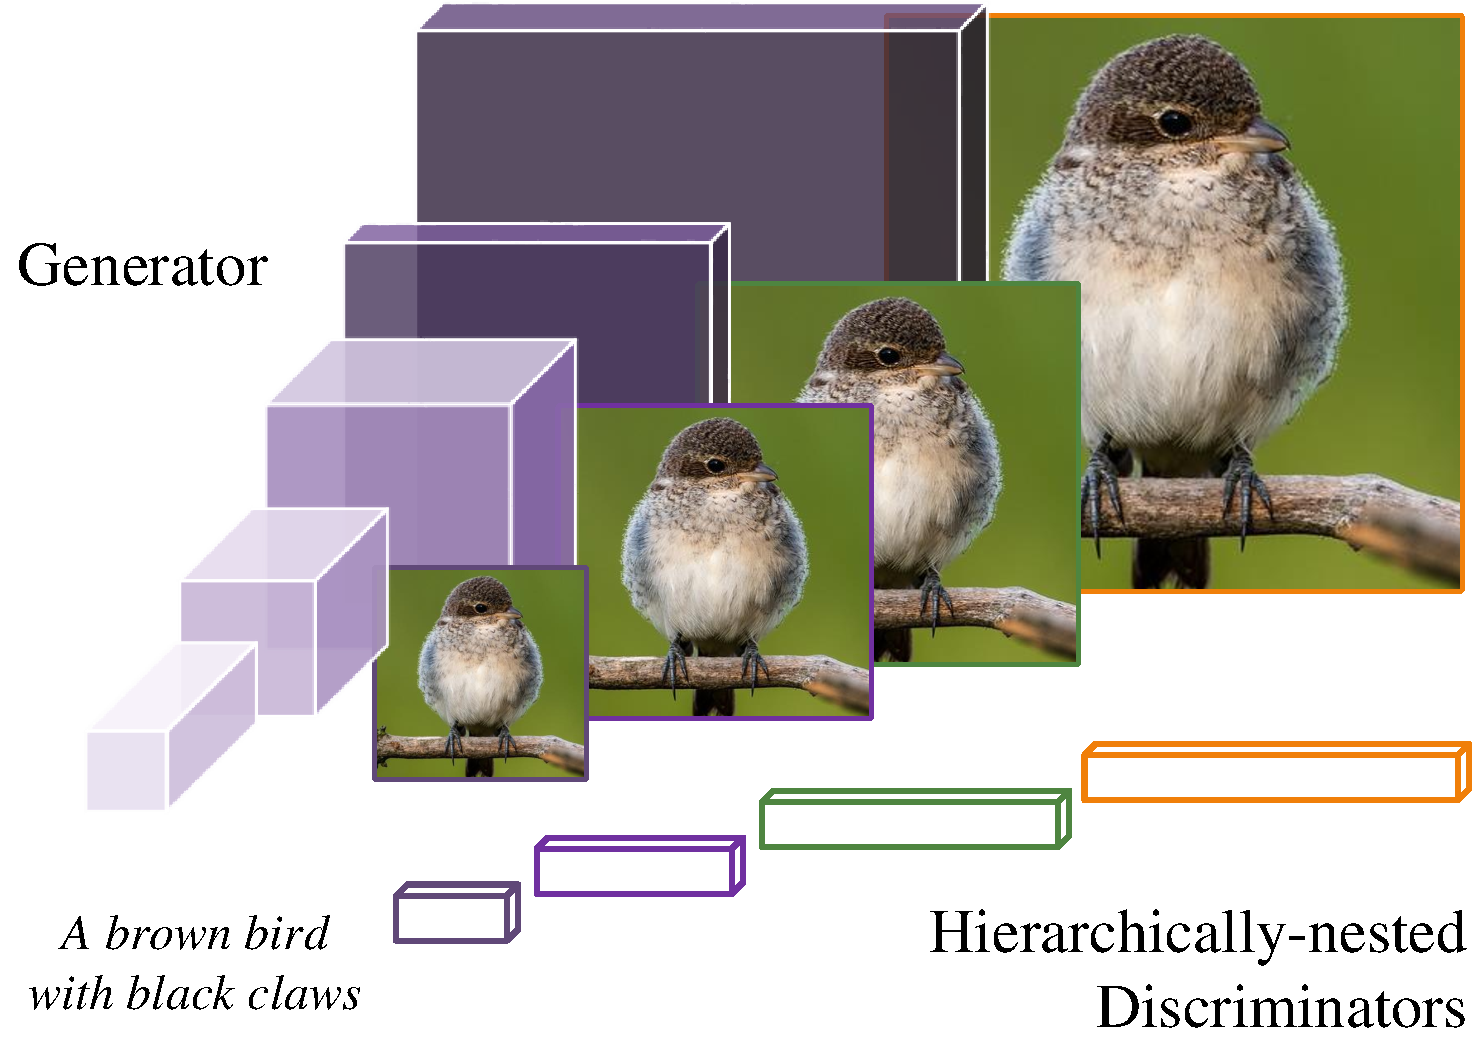
\includegraphics[width=0.4\textwidth]{figure/intro.pdf}
%	\vspace{-.3cm}
%	\caption{Overview of our hierarchically-nested adversarial network. It contains a single-stream generator and several nested discriminators along the depth dimension of the generator, which can generate high-resolution images conditioned on a sentence.} \label{fig:archs-review} \vspace{-.3cm}
%\end{figure}
%\begin{figure}[t]
%	\centering
%	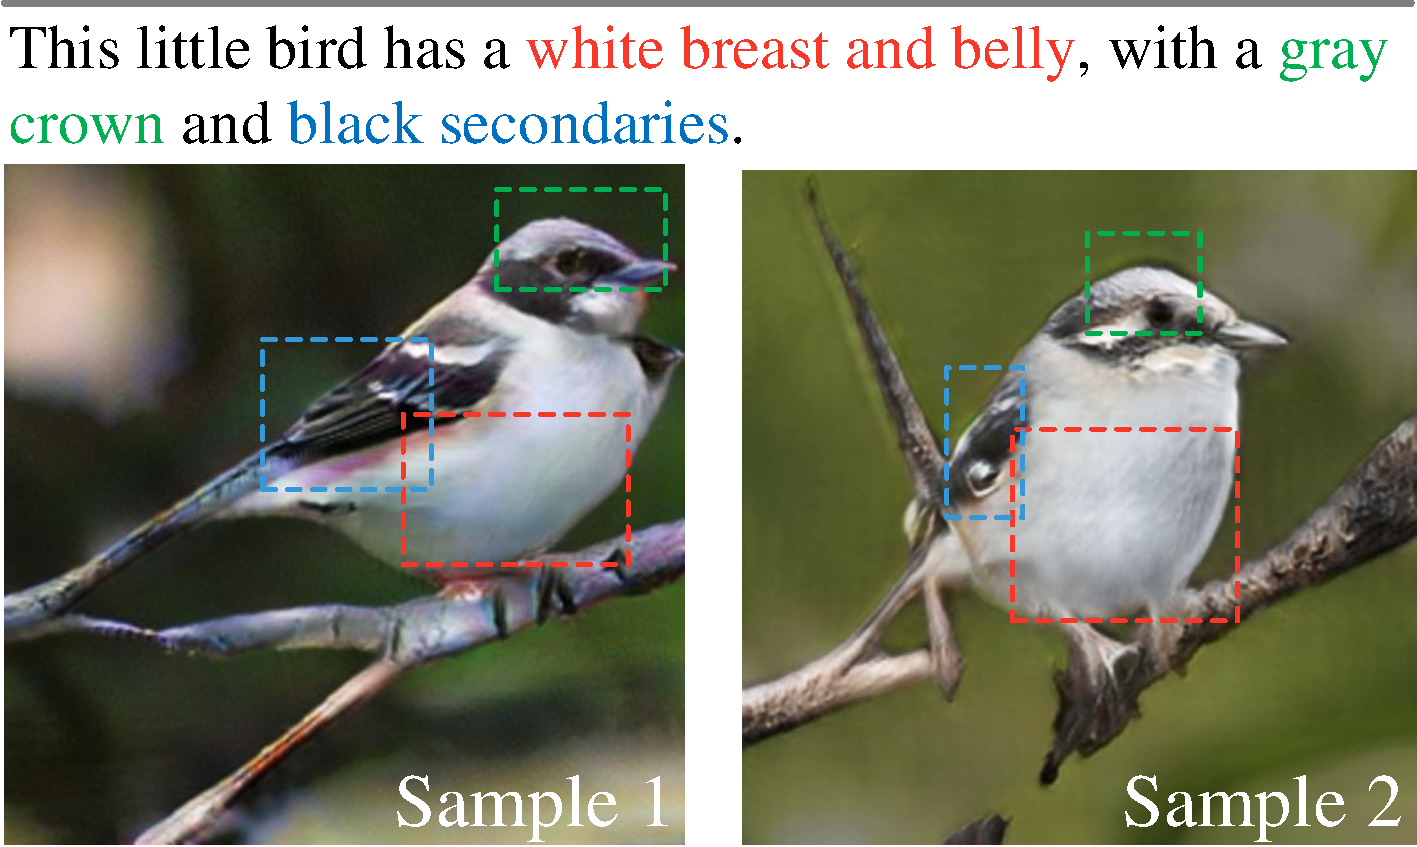
\includegraphics[width=0.4\textwidth]{figure/single_view.pdf}
%	\vspace{-.3cm}
%	\caption{Overview of our hierarchically-nested adversarial network. It contains a single-stream generator and several nested discriminators along the depth dimension of the generator, which can generate high-resolution images conditioned on a sentence.} \label{fig:archs-review} \vspace{-.3cm}
%\end{figure}
Generative adversarial networks (GANs) have become the main solution to this task. 
Reed \etal \cite{reed2016generative} address this task through a GAN based framework. But this method only handles image up to $64^2$ resolution and can barely generate vivid object details.
Based on this method, Zhang \etal \cite{han2017stackgan} present a successful two-state training approach (StackGAN) by stacking another low-to-high resolution GAN to generate high-quality $256^2$ images. Later on, Dong \etal \cite{dong2017semantic} propose to bypass the difficult of translate vector embedding to RGB images and treat it as an pixel-to-pixel translation \cite{isola2016image}, by re-rendering an arbitrary-style training ($128^2$) image conditioned on a targeting description. But its high-resolution synthesis ability is unclear. 
At present, how to train from the low-dimensional text space to synthesize high-resolution and diverse images in a fully end-to-end manner is still an open and attractive question. 

%We outline several empirical reasons for the challenges of 
Text-to-image synthesis using GANs has two main difficulties. The first is the fundamental problem of balancing the convergence between generators and discriminators \cite{goodfellow2014generative,improvedGAN}. %How to utilize the multimodal information between images and text in discriminator is extremely important to generate effective gradients. 
The second is stably modeling the huge pixel space in high-resolution images \cite{han2017stackgan}. 
An effective strategy to regularize generators is critical to help capture the complex image statistics \cite{huang2016stacked} as well as guarantee semantic consistency. 
%The first reason is that the pixel space in high resolution image is substantially large \cite{han2017stackgan}. 
% Keeping semantic consistency as well as diversity
%The first reason comes from the fundamental difficulty of balancing the stability between generators and discriminators. There are a rich number of literature trying to stabilize GAN training \cite{salimans2016improved} and regularize networks \cite{huang2016stacked}. 
%But especially for text-to-image synthesis, how to utilize the multimodal information between images and text in discriminator is extremely important and needs careful consideration. The second reason is that the pixel space in high resolution image is substantially large \cite{han2017stackgan}. Keeping semantic consistency as well as diversity in generated images needs more specialized designs for discriminators to generate effective gradients, as well as generators to prevent gradient vanishing. 
With careful consideration of these problems, in this paper, we propose a novel end-to-end method that can directly model high-resolution image statistics and generate semantically consistent and photographic image (see Figure \ref{fig:intro}). The contributions are described as follows.


Our generator resembles a simple vanilla GAN, without requiring any internal text conditioning like \cite{han2017stackgan} or outside image annotation supervision like \cite{dash2017tac}. To tackle the problem of the big leap from the text space to the high-resolution image space, our insight is to leverage and regularize hierarchical representations with additional deep adversarial constraints. 
We introduce accompanying hierarchically-nested discriminators at multi-scale intermediate layers to play adversarial games and thereby encourage the generator approaching the real training data distribution. 
We also propose a novel convolutional neural network (CNN) framework for the generator to cooperate with our nested discriminators more effectively.
To guarantee the image diversity and semantic consistency,
\textcolor{red}{we enforce nested discriminators at different hierarchies to simultaneously differentiate real-and-fake image-text pairs as well as real-and-fake global images or local image patches with certain focal ranges.}
This multi-purpose conditional adversary is mutually beneficial to allow each focus on its respect duty. 
%% It is a regularization to limit the discriminators to use unexpected information to make decision. 

We validate our proposed method on three datasets, CUB birds \cite{welinder2010caltech}, Oxford-102 flowers \cite{Nilsback08}, and large-scale MSCOCO \cite{lin2014microsoft}. In complement of existing evaluation metric (inception score \cite{improvedGAN}) for generative models, we also introduce a new visual-semantic similarity metric to evaluate the alignment between generated images and conditioned text. Extensive experimental results and analysis demonstrate the effectiveness of our method and significantly improved performance compared against previous state of the arts on three metrics. All source code will be released.


\begin{figure*}[t]
	\centering
	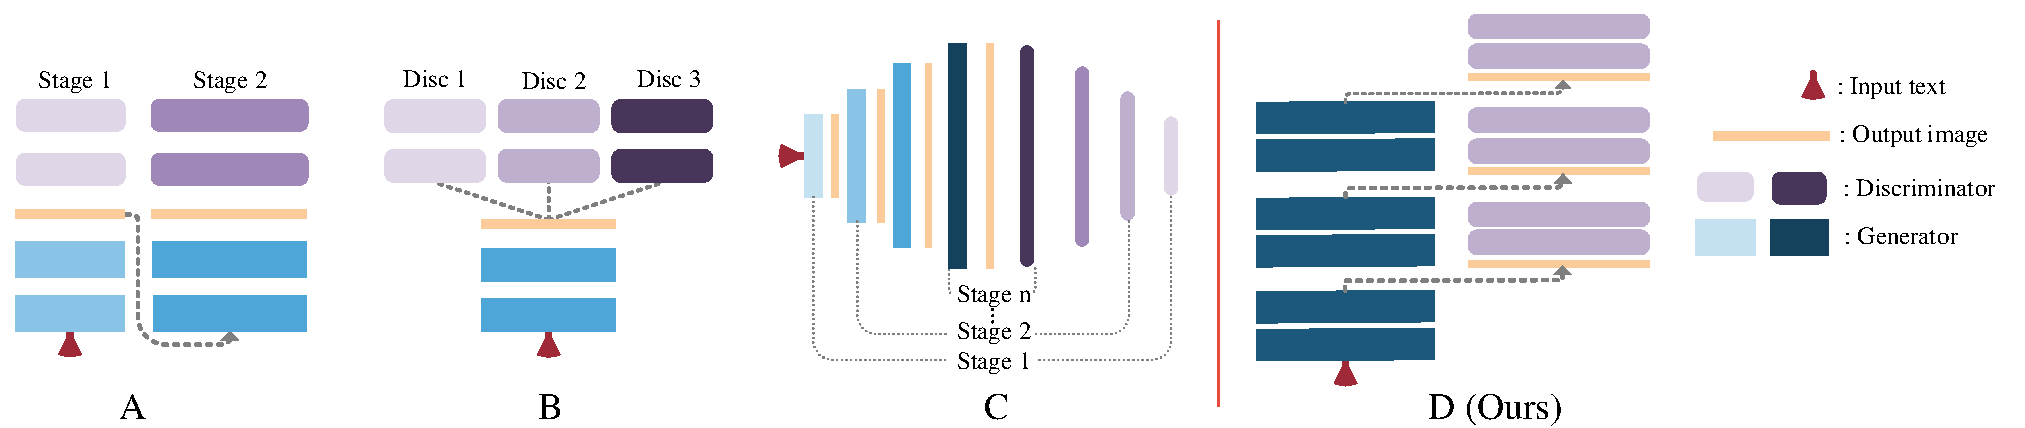
\includegraphics[width=0.95\textwidth]{figure/views2.pdf}
	\vspace{-.2cm}
	\caption{Overviews of some typical GAN frameworks. \textbf{A} uses multi-stage GANs \cite{han2017stackgan,denton2015deep}. \textbf{B} uses multiple discriminators with one generator \cite{durugkar2016generative,tu_etal_nips17_d2gan}. \textbf{C} progressively trains symmetric discriminators and generators \cite{Karras2017progressive,huang2016stacked}. \textbf{A} and \textbf{C} can be viewed as decomposing high-resolution tasks to multi-stage low-to-high resolution tasks.  \textbf{D} is our proposed framework that uses a single-stream generator with hierarchically-nested discriminators trained end-to-end.} \label{fig:archs-review}
\end{figure*}


\section{Related Work}
We discussed related work and further clarify the novelty of our method by comparing with them.

Deep generative models attract wide interests recently, including GANs \cite{goodfellow2014generative}, Variational Auto-encoders (VAE) \cite{kingma2013auto}, etc \cite{oord2016pixel}. 
There are substantial existing methods investigating better usage of GANs for different applications, such as image synthesis \cite{radford2015unsupervised, shrivastava2016learning}, (unpaired) pixel-to-pixel translation \cite{isola2016image,zhu2017unpaired}, medical applications \cite{costa2017towards}, etc \cite{ledig2016photo,huang2016stacked}.

Text-to-image synthesis not only requires diverse and high-quality image generation but also requires precise semantically consistent mapping in the image space.  Reed \etal \cite{reed2016generative}  is th first to introduce a method that can generate $64^2$ resolution images, which is similar with DCGAN \cite{radford2015unsupervised}. This method presents a new strategy for image-text matching aware adversarial training. Reed \etal \cite{reed2016learning} propose generative
adversarial what-where network (GAWWN) to enable location and content instructions in text-to-image synthesis. StackGAN \etal \cite{han2017stackgan} propose a two-stage stacking GAN training approach that is able to generate $256^2$ compelling images. Recently, Dong \etal \cite{dong2017semantic} propose to learn a joint embedding of images and text so as to re-render a prototype image conditioned on a targeting description. Cha \etal \cite{char2017perceptual} explore the usage of the perceptional loss with a CNN pretrained on ImageNet \cite{johnson2016perceptual} and Dash \etal \cite{dash2017tac} make use of auxiliary classifiers (similar with \cite{odena2016conditional}) to assist GAN training for text-to-image synthesis. 
	
Learning a continuous mapping from a low-dimensional embedding manifold to a complex real data distribution is a long-standing problem. Although GANs have made significant progress, there are still many unsolved difficulties, e.g. training instability and high-resolution extensions. Wide methods have been proposed to address the training instability, such as various training techniques \cite{salimans2016improved,arjovsky2017wasserstein,berthelot2017began,shrivastava2016learning,odena2016conditional}, regularization using extra knowledge (e.g. image labels, ImageNet CNNs, etc) \cite{dosovitskiy2016generating,ledig2016photo,dash2017tac,dash2017tac}, or different generator and discriminator combinations  \cite{metz2016unrolled,durugkar2016generative,yang2017lr,huang2016stacked}. \textit{While our method shows a new way to unite generators and discriminators and does not use any extra information apart from training paired text and images.} Additionally, it is easy to see the training difficulty increases significantly as targeting image resolution increases.

%for example, label smoothing and discriminator feature matching \cite{salimans2016improved, }, training stronger discriminator is beneficial to encourage generators \cite{arjovsky2017wasserstein}. Balancing through a equilibrium enforcing method \cite{berthelot2017began}
%Preventing discriminators from forgetting past samples and re-introduces artifacts \cite{shrivastava2016learning}. Increasing the information richness in GANs has been shown very useful \cite{odena2016conditional}.  

To synthesize high-resolution images, cascade networks are useful to decompose original difficult tasks to multiple subtasks (Figure \ref{fig:archs-review} A).
Denton \etal \cite{denton2015deep} train a cascade of GANs within a Laplacian pyramid framework (LAPGAN) and use each to generate difference images, conditioned on random noises and the output from the last pyramid level, and thereby push up the output resolution through by-stage refinement. StackGAN also shares similar strategy with LAPGAN. Following this strategy, Chen \etal \cite{chen2017photographic} present a cascaded refinement network to synthesize high-resolution scene from semantic maps. 
%%Huang \etal \cite{huang2016stacked} propose a top-down stacked GAN to leverage mid-level representations, which shares some similarities with StackGAN and our method. However, this method needs multiple symmetric bottom-up pre-trained discriminators and the usage for high-resolution image is unclear. 
Recently, Karras \etal \cite{Karras2017progressive} propose a progressive training of GANs for very high-resolution image generation (Figure \ref{fig:archs-review} C). \textit{Compared with these strategies that train low-to-high resolution GANs progressively, our method has advantages of leveraging mid-level representations to encourage implicit subtask integration, which makes end-to-end high-resolution image synthesis in a single vanilla-like GAN possible.}

%More advantages of our method compared with others will be demonstrated in the following.

Leveraging hierarchical representations of neural networks is an effective way to enhance implicit multi-scaling and ensembling for tasks such as image recognition \cite{lee2015deeply} and pixel or object classification \cite{xie2015holistically,cai2016unified,long2015fully}. Particularly, using deep supervision \cite{lee2015deeply} in hierarchical convolutional layers is shown to be ablue to increase the discriminativeness of feature representations. 
\textit{Our hierarchically-nested adversarial objective is inspired by these families of CNNs with deep supervision. }
%Our proposed hierarchically-nested adversarial supervision enhances layer representations to support final high resolution outputs.   

%
%
%\subsection{Summarize different architectures}
%refer to HED.

%\section{Preliminary}
%\subsection{Generative Adversary Network}
%Generative adversary networks (GANs) are composed of a generator $G$ and a discriminator $D$, which are alternatively trained to compete with each other in a two-player minimax game. The discriminator $D$ is optimized to distinguish the synthesized images from the real images, meanwhile, the generator $G$ is trained to fool the discriminator by trying to convert an input distribution $p_z$ to the true data distribution $p_{data}$. Concretely, the overall training procedure can be analogous to the following two-player min-max game $V(D, G)$, where the optimal $G$ and $D$ can be obtained by 
%\begin{equation}
%\label{equ:GAN}
%\begin{split}
%G^*, {D}^* = \arg~\underset{G}{\min}\ \underset{\mathcal{D}}{\max}~ V(D, G)
%\end{split}
%\end{equation}
%
%%\begin{equation}
%%\label{game}
%%\begin{split}
%%\underset{G}{\min}\ \underset{D}{\max}\ V(D, G) =  &\mathbb{E}_{x\sim p_{data}}[\log D(x)] +  \\
%%&\mathbb{E}_{z\sim p_{z}}[\log (1-D(G(z)))]		   
%%\end{split}
%%\end{equation}
%%where $x$ is a real image sampled from the true data distribution $p_{data}$, $z$ is a noise vector usually sampled from some predefined distribution $p_{z}$ (e.g., Gaussian distribution).
%%In practice, It's been shown to work better for the generator $G$ to minimizing $-\log(D(G(z)))$ rather than $\log(1-D(G(z)))$, namely, the $\log(D)$ trick.
%%In this paper, we replace the negative log likelihood loss with a least square objective\cite{lsgan}. 
%
%Conditioned GAN \cite{isola2016image} is a variation of traditional GAN where both the generator network $G$ and discriminator network $D$ are conditioned on an additional condition vector besides the noise vector. In this paper, we consider the task of training a deep  generative adversarial network conditioned on the embedding of the text descriptions of the images.


\section{Method}
%Figure \ref{fig:archs} illustrate the overall method.

\subsection{Adversarial objective basics}
In brief, the two-player game in GANs \cite{goodfellow2014generative} is played by a generator $G$ network and a discriminator $D$ network, which are alternatively trained to compete with each other and thereby improve each other. The discriminator is optimized to distinguish synthesized images from real images, meanwhile, the generator is trained to generate realistic images to fool the discriminator. Concretely, the overall min-max optimization objective is defined as: 
%where the optimal $G$ and $D$ can be obtained by 
%The discriminator is optimized to distinguish synthesized images from real images, meanwhile, the generator is trained to fool the discriminator and transform an input distribution $p_z$ to the true data distribution $p_{data}$. Concretely, the overall training procedure can be analogous to the following two-player min-max game $\mathcal{L}(D, G)$, where the optimal $G$ and $D$ can be obtained by 
\begin{equation}
\label{equ:GAN}
\begin{split}
G^*, D^* = \arg~\underset{G}{\min}\ \underset{D}{\max}~ \mathcal{V}(D, G, Y, \bm z),
\end{split}
\end{equation}
where $Y$ denotes training images and $\bm z\sim\mathcal{N}(0,1)$ denotes a random noise. The value function $\mathcal{V}$ aims to minimize the Jensen-Shannon divergence between the data and the model distribution. $G$ is learned to approximate $G(\bm z) \sim p(Y)$.  The loss $\mathcal{L}$ for the valuation function is usually a cross-entropy loss, such that $\mathcal{V}(\cdot) = - \mathcal{L}(\cdot)$. 


%Conditioned GAN \cite{isola2016image} is a variation of traditional GAN where both the generator network $G$ and discriminator network $D$ are conditioned on an additional condition vector besides the noise vector. In this paper, we consider the task of training a deep generative adversarial network conditioned on the embedding of the text descriptions of the images.

%To generate high-resolution photo-realistic images from text embeddings, we propose a simple and effective Hierarchically-nested Generative Adversarial Network.
%Our approach is to train both generator and discriminator conditioned on sentence embedding vectors. We leverage functional loss for discriminator and hierarchically nested side outputs as hierarchical supervision for both generator and discriminator to achieve our goal of generating photo-realistic images from text descriptions.  
%
%In general, the generator takes text embedding and random noise vector as input and synthesis images at different scales (e.g, $64\times64$, $128\times128$, $256\times256$). The discriminator, on the other hand, is trying to judge the pair of synthesized images and the corresponding text embedding as fake pairs as well as differentiating the real images from the fake images. $G$ and $D$ are optimized alternatively until converges.
%
%
%\textbf{Notation } 
%We denote the training data set by $S=\{({X}^n, {T}^n),n=1,...,N\}$, where $X^n$ is the $n-$th training image, and $T^n={t^1,...,t^m}$ as $m$ text descriptions corresponds to $X^n$. 
%
%Since we obtain the text embedding vector using the per-trained char-rnn text encoder provided in \cite{reed2016generative}. For simplicity, we do not differentiate text description and it's corresponding text embedding vector in this paper.  Our goal is to learn a generator $G$ that could produce high resolution images of high visual quality as well as variability giving an input text description $t$.  
%
%The input to $G$ compress input sentence embedding, and one noise input.
%Denote the image dimension, text embedding dimension and the dimension of the noise input as $I$, $T$ and $Z$, respectively. Please note that, $G$ has multiple branches and generates multiple images of different sizes. For each image size, we have a distinct discriminator $D$ associated with it. 
%%For simplicity, we only describe one image size.  
%
%The generator is denoted $G: \mathcal{R}^{Z}: \times \mathcal{R}^{T}\rightarrow\mathcal{R}^{I}$, the image discriminator $D_{img}: \mathcal{R}^{I}\rightarrow\{0, 1\}$, and the matching-aware pair discriminator $D_{pair}: \mathcal{R}^{I}: \times \mathcal{R}^{T}\rightarrow\{0, 1\}$. 
%
%\textbf{Variational text embedding } Following the practice of \cite{han2017stackgan}, instead of using the plan deterministic non-linear transformation of the original $t$, we obtain the conditional vector $c$ by sampling from a Gaussian distribution $\mathcal{N}(\mu(t), \Sigma(t) )$, in which the mean $\mu(t)$ and the diagonal covariance matrix $\Sigma(t)$ are non-linear transformation of the original text embedding $t$. This type of conditional augmentation technique can be used to inject randomness into the text embedding vector $t$ to mitigate the common problem that conventional conditional GAN training paradigm usually learns to totally ignore the randomness, resulting to collapsing results lacking diversity \cite{reed2016generative}. In addition, using this kind of text embedding makes the input pure stochastic, making it more difficult for the generator to over fit the training data.

\subsection{Hierarchical-nested adversarial objectives}
%Directly predicting high resolution synthesized images are challenging, not only because of the difficulties in training but also due to the large variation and instability in the hidden layers.
Numerous methods have demonstrated ways to unite generators and discriminators for image synthesis. Figure \ref{fig:archs-review} and Section 2 discuss some typical frameworks.
Our method actually explores a new dimension of playing this adversarial game along the depth of a CNN (Figure \ref{fig:archs-review} D), which integrates additional discriminators at mid-level features of the generator $\mathcal{G}$. 
The hierarchically-nested objectives 
%We conjecture that adding hierarchical adversarial objective using side outputs can
act as regularizers to the hidden space of $\mathcal{G}$, which can reduce the training instability and also offer a short path for better error signals.

The proposed $\mathcal{G}$ is a CNN (defined in Section 3.4) with side outputs:

%This architecture resemble the proposed inverse architectures in edge detection\cite{xie2015holistically} and classification \cite{lee2015deeply}, which demonstrate that additional supervision to hidden layers can improve model generalization and boost optimization.  
\begin{equation}
\label{side}
X_1,..., X_s = \mathcal{G}(\bm t, \bm z), 
\end{equation}
where  $\bm t\sim p(data)$ denotes a sentence embedding vector in the real training data distribution (generated by a text character encoder). $\mathcal{G}$ produces $s-1$ side outputs (size-growing images) and a final output $X_s$ with the highest resolution.

%$\mathcal{X}^i = \{X^i_1, .. X^i_s\}$ are side output
%Given $z\in \mathcal{R}^{Z} \scriptsize{\sim} \mathcal{N}(0,1)$ and a text description embedding $t$, 
%$G$ generates $s$ side outputs using intermediate layers, $o=\{o_1,...,o_s\}$,
%Note that the dimension of $o_1,..,o_s$ increases according to the resolution
%(e.g., 64$\times$64, 128$\times$128, and 256$\times$256). 
%Denote $\mathcal{X}^i = \{X^i_1, .. X^i_s\}$ as the pyramid of resized images constructed from original image $X^i$.  
%Denote $\mathcal{D}=\{D_1, ..., D_o\}$ as the whole set of discriminators.
%e aim to solve the following optimization problem:

For each side output $X_i$, we propose to apply a discriminator $D_i$ to perform independently adversarial games. Therefore, our full min-max objective is defined as 
\begin{equation}
\label{equ:optim}
\begin{split}
  \mathcal{G}^*, \mathcal{D}^*&  =  \arg~\underset{G}{\min}\ \underset{\mathcal{D}}{\max}~ \mathcal{V}(\mathcal{G},\mathcal{D}, \mathcal{Y}, \bm t, \bm z), \\
  \text{where} \;\;	 \mathcal{D} & \in  \{D_1, ..., D_s\}, \; \mathcal{Y} = \{Y_1, ..., Y_s\},
\end{split}
\end{equation}
where $ \mathcal{Y}$ contains a set of training images at multi-scales, $\{1,...,s\}$.
%where $\mathcal{D}$ contains the optimal discriminators $\{D_1^*, ..., D_o^*\}$, and $ \mathcal{L}(G,\mathcal{D}, \bm{X}, \bm{T} )$ is the full objective of this mini-max game.
%Please note that in this setting, 
Compared with Eq. (\ref{equ:GAN}), one generator competes with multiple discriminators  $\{D_i\}$ at different hierarchies (Figure \ref{fig:archs-review} D), where each focus on learning diverse discriminative features in different contextual scales.
%%Discriminators do not share weights with each other, which offers them full flexibility to focus on learning diverse discriminative features in different contextual scales.
In principle, the lower-resolution side output is forced to learn semantic consistent image structures (e.g., object sketch, color, and background), and the subsequent higher-resolution side outputs are used to render details to the images. Since the model is trained in an end-to-end fashion, the lower-resolution outputs can fully enjoy top-down knowledge from higher resolutions. We hypothesize such consistency reduces the model instability.
As an evidence, we can obtain significantly more consistent information exhibited in both low- and high-resolution outputs compared with StackGAN (see experiments). 
%%We present the following multi-purpose adversarial loss to support more effective generator training. 


\subsection{Functional adversarial losses}
Our generator produces size-growing side outputs which compose an image pyramid. 
We leverage this hierarchy property and allow adversarial losses to be multi-purpose to capture different (conditioned and unconditioned) statistics, with a goal to guarantee both semantic consistency and image fidelity. 

To guarantee semantic consistency, we adopt the matching-aware pair loss proposed by \cite{reed2016generative}. The discriminator is designed to take image-text pairs as inputs and trained to identify two types of fakes: real image with mismatched text and fake image with conditioned text.

The pair loss is designed to guarantee the global semantic consistency. However, there is no explicit loss that forces the discriminator to differentiate real images from fake images. As the image resolution goes higher, discriminators might loss focus for local fine-grained image details.
%However, this loss has two major weaknesses. First, there is no explicit loss that force the discriminator to differentiate real images from fake images. 
%Combining both tasks (generating realistic images and matching image with text) into one output further complicates the learning tasks, which is already challenging. 
%Second, as the image resolution goes higher, it might be challenging for a global pair-loss discriminator to capture local fine-grained details.  
In addition, as pointed in \cite{shrivastava2016learning}, a single global discriminator may over-emphasize certain unexpected image features and lead to artifacts. 

To guarantee image fidelity, our solution is to add local adversarial image losses on image patches. 
%The insights are two folds:
%\begin{itemize}\vspace{-.1cm}
%\setlength\itemsep{-0.3em}
%\item Further forcing the generated samples to have only only global but also local similar statistics to real image patches, which is beneficial for rendering fine-grained details. 
%
%\item \textcolor{red}{Image loss without using paired text can be beneficial in the sense that it focus more on image information. The richness of discriminator supervision usually has advantages for generalization. } 
%\vspace{-.2cm}
%\end{itemize}
We expect the low-resolution discriminator to focus on global structures, while high-resolution outputs focus more on local image details. Therefore, through the pyramid of the size-growing side outputs, we configure the focal range (the size of each non-overlapping image patch need to classify) to be also growing.
The local image adversarial loss is implemented as a fully CNN \cite{shrivastava2016learning,zhu2017unpaired}.  
Figure \ref{fig:loss} illustrates how hierarchically-nested discriminators compute the two losses on generated images. 

\begin{figure}[t]
	\centering
	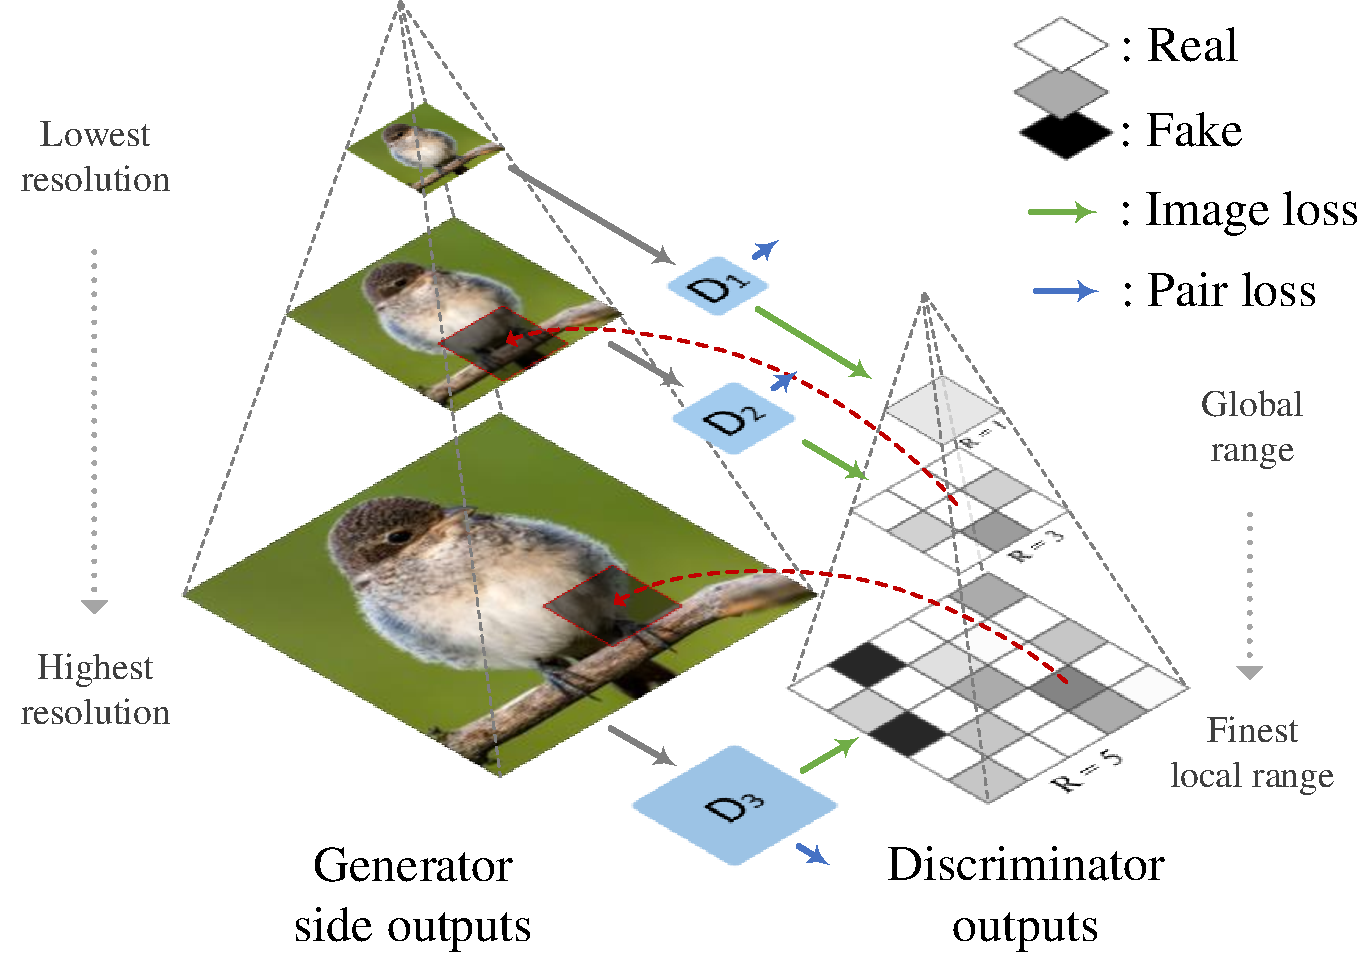
\includegraphics[width=0.49\textwidth]{figure/loss.pdf}
	\vspace{-.5cm}
	\caption{Given a set of images from the side output pyramid of the generator, the corresponding discriminator $D_i$ computes the matching-aware pair loss and adaptive local image loss (outputting a $R{\times}R$ probability map to classify real or fake patches). The focal range decreases as the image size grows. }  \vspace{-.3cm}
	\label{fig:loss}
\end{figure}


\textbf{Full Objective } Overall, our hierarchically-nested discriminators $\{D_i\}$ minimize the following loss\footnote{The objective of the generator is omitted as it can be easily inferred.}:
\vspace{-.2cm}
\begin{equation}
\begin{split}
\mathcal{L}(& \mathcal{G}, \mathcal{D})  = \sum_{i=1}^{s} \Big(  L_2\big(D_i({Y}_i)\big) +  L_2\big(D_i({Y}_i, \bm t_{Y})\big) \, + \\ 
& \overline{L_2}\big(D_i({X}_i)\big)  + \overline{L_2}\big(D_i({X}_i, \bm{t}_{X_i})\big) + \overline{L_2}\big(D_i({Y}_i,  \bm{t}_{\overline{Y}})\big) \Big),
\end{split}
\end{equation}
where $L_2(x) = (x - \mathbb{I})^2$ is the mean-square loss (instead of the conventional cross-entropy loss) and $\overline{L_2}(x) =x^2$. For local image loss with varying focal ranges, the shape of $x, \mathbb{I} \in \mathbb{R}^{R{\times}R}$ varies accordingly (see Figure \ref{fig:loss}). $R=1$ refers to the (largest local) global range. For the matching-aware pair loss, 
$\{Y_i, \bm t_{Y}\}$ denotes a matched image-text pair and $\{Y_i, \bm{t}_{\overline{Y}}\}$ denotes a mismatched image-text pair.

Furthermore, this separation of the image loss from the matching loss in our method opens further possibilities, such as utilizing the unlabeled image to improve both the generator and discriminator.
\textcolor{red}{In the spirit of variational auto-encoder \cite{vae} and the practice of StackGAN \cite{han2017stackgan}, namely conditioning augmentation (CA), we sample the input text $\bm t$ from a Ganssian distribution $\mathcal{N}(\mu({\bm t}), \Sigma({\bm t}))$, where $\mu$ and $\Sigma$ are functions of $\bm t$ (learned with the network), which produces a $256$-d text input.
We add the Kullback-Leibler divergence regularization term, $D_{KL}(\mathcal{N}(\mu({\bm t}), \Sigma({\bm t}) )|| \mathcal{N}(0, \bm{I}))$ \cite{vae}, to the $G$ loss to force the smooth sampling over the text embedding distribution. }


%\begin{equation}
%{\small 
%\label{equ:pariG}
%\begin{split}
% \mathcal{L}(\mathcal{G}, \mathcal{D})  = & \mathbb{E}_{ t \sim p_{t}, z \sim p_{z}  , X \sim p_{\mathcal{G}(t, z)}} \Big[ \\
%&   \sum_{i=1}^{s} \big( M(D_i({X}_i)) + M(D_i({X}_i, \bm t)) \big)  + \\
%&   \sum_{i=1}^{s} \big( \hat{M}(D_i({X}_i)) + \hat{M}(D_i({X}_i, \bm t)) \big) \Big] 
%\end{split}
% }
%\end{equation}

%\begin{equation}
%\label{equ:totalG}
%\begin{split}
%\mathcal{L}_{g}(G,o,\hat{o}, t)  = &  \mathcal{L}_{pair}(G) + \frac{\alpha}{2}~(\mathcal{L}_{local}(G, o) + \mathcal{L}_{local}(G, \hat{o})) + \\
%& \beta~D_{KL}(\mathcal{N}(\mu({t}), \Sigma({t}) )|| \mathcal{N}(0, \bm{I})) 
%\end{split}
%\end{equation}



%In addition, at the very beginning of the training,  generated images are usually far away from true image distribution, the discriminator can very easily judge a pair as invalid without using much pair information. \textcolor{red}{need more explanationn.}
%We not only want the whole image is classified as true image by the discriminator, but also want to restrict the discriminator to classify all the local patches of high resolution output as true as well.   

%so that they can focus more on local details, we restrict the receptive field of the image discriminator.

%\subsection{Matching Aware Pair-Loss}
%During the setting of conditional generative adversarial learning, simply generating images of high visual quality is not enough, most importantly, we want the generated images well aligned with the conditioning information (ie, text description in our model).     
%Given a pair of image and text embedding $(x, \psi{t})$ as input, in the discriminator $D_i$, we first transfer $x$  to an image code $Code_x$. $Code_x$ along with $f_{sent}(\psi_t)$ is concatenated and fed to the matching aware branch to compute a final scale value indicating the probability of the pair being real or fake, where $f_{sent}$ consists of one linear layer and one leaky ReLU transformation,  the matching-aware branch is a set of residual blocks with strid-2 convolution, more details of the architecture will be provided in the appendix. Besides that, the image code is also fed to an image-disc branch, whose structure is very similar to the matching-aware branch, to judge the probability of the input image being real or fake. We performance batch normalization on all convolutional layers. \textcolor{red}{like stackgan, I will add much more architecture details later}  
%
%The generator $G$ and discriminator $D$ are optimized alternatively using their corresponding loss function. 
%Therefore, the discriminator are designed to take image and sentence pair as input and should be able to identify two types of errors: real image with mismatch conditional text information and fake image with real text. In our case, the discriminator is explicitly trained with three pair configurations, namely: real image with right text as positive training sample, and the aforementioned two sources of error pairs as negative training samples. 

%Given a mini-batch of training data consists of images $X$ and the corresponding text $t$, mismatching text $\hat{t}$. For simplicity, we omit the batch index.  To train the discriminator,  we also need to sample fakes images $o_i$ using $G$. For the $i-$th discriminator $D_i$ , we can have:

%\begin{equation}
%\label{equ:matchignloss}
%\begin{split}
%\mathcal{L}_{pair}(D_i)  = & \mathbb{E}_{(X_i, \hat{t}) \sim p_{data}}[(D_i( {X_i},  {t}) - 1) ^ 2 ] - \frac{1}{2}*\\ 
%&   \mathbb{E}_{(X_i, \hat{t}) \sim p_{data}}[(D_i({X_i}, \hat{{t}}) - 1)^2  ] - \frac{1}{2} *\\
%&   \mathbb{E}_{t \sim p_{data}}[ (D_i( {o}_i, {t}))^2 ]  
%\end{split}
%\end{equation}
%
%Similarly, the pair wise objective of generator can be summarized as:
%\begin{equation}
%\label{equ:pariG}
%\begin{split}
%\mathcal{L}_{pair}(G)  = & \sum_{i=1}^{s} ( \mathbb{E}_{t \sim p_{data}}[ (D_i( {o}_i, {t}) - 1) )^2 ] )
%\end{split}
%\end{equation}
%
%where $o_i$ is the $i-$th output of the $G$,  this type of loss is used to push the valid image-text pair away from the invalid pairs.
%
%\subsection{Local Adversarial Image Loss}
%%As is shown in Figure. \ref{overview}, the discriminator $D$ in our model mainly consists of two branches: matching-aware pair discrimination branch $D_{pair}$, and image discrimination branch $D_{img}$, both branches share the same  image encoder.
%
%The pair-loss is designed to differentiate invalid pairs from valid ones.
%It works by first translating the image to a compact size code, then the image code and the sentence vector is concatenated and fed to successive layers to predict the validity of the input image-sentence pair. 
%
%Overall, the pair loss is designed to capture the global context semantic information.  However, this loss has two problems, firstly,  there is no explicit loss that push the discriminator to differentiate real images from the fake images. Combining both tasks (generating realistic images and matching image with text) into one output further complicates the learning tasks, which is already challenging. Second,  as the image resolution goes higher, it might be challenging for the global pair wise discriminator to capture local fine-grained details.  In addition, as is also pointed in \cite{shrivastava2016learning}, a single global strong discriminator tend to over-emphasize certain image feature and may lead to artifacts. 
%
%%More specifically, ideally the image patches sampled from the higher resolution outputs 
%
%Our solutions is to add hierarchical local adversarial image loss which does not require sentence information, to all the side outputs. To make the image discriminator focus more on local details, we restrict the receptive field of the image discriminator.
%Our insight has two folds:
%\begin{itemize}
%	\item 1. Forcing the local patch of generated samples to have similar statistics to real image patch can be beneficial to rendering fine-grained details. %
%	 
%	\item 2. Image loss without using pair sentence information can be beneficial in the sense that it utilize more information as well as it directly push the generated image to the true image distribution. We hypothesis this type of loss can help the model to stabilize and boost the training. 
%\end{itemize}
%%In addition, at the very beginning of the training,  generated images are usually far away from true image distribution, the discriminator can very easily judge a pair as invalid without using much pair information. \textcolor{red}{need more explanationn.}
%%We not only want the whole image is classified as true image by the discriminator, but also want to restrict the discriminator to classify all the local patches of high resolution output as true as well.   
%Since our model generates a pyramid of outputs with increasing image sizes. 
%We expect the low resolution output capture the global structure and color information, while the higher resolution outputs focus on local image details. 
%
%To force the discriminator focus on the fine-grained details, a nature way is to fix the receptive field for all the generator. To this end, we propose a hierarchical image loss, where the output of image  discriminator is a grid of values. 
%
%Denote $K_i$ as the $i-$th local image discriminators,  the output $d_i = K_i(X_i)$ has a size increasing with input $X_i$. For instance 1$\times$1 for 64$\times$64 input, 4$\times 4$ for 128$\times$128 and 8$\times 8$ for 256$\times$256 etc.  In this way, even the resolutions goes higher, the receptive field keeps unchanged.  Specifically, the proposed local image loss can be given by:
%\begin{equation}
%\label{equ:local}
%\begin{split}
%\mathcal{L}_{local}(K_i, X_i, o_i, t )  = & \mathbb{E}_{(x, t) \sim p_{data}}[ \mathbb{E}(K_i( {X_i}) - 1) ^ 2 ] - \\
%&  \mathbb{E}_{t \sim p_{data}}[  \mathbb{E}(K_i( {o}_i))^2 ]  
%\end{split}
%\end{equation}
%
%Similarly, the pair wise objective of generator can be summarized as:
%\begin{equation}
%\label{equ:pariG}
%\begin{split}
%\mathcal{L}_{local}(G, o)  = & \sum_{i=1}^{s} ( \mathbb{E}_{t \sim p_{data}}[ \mathbb{E} (K_i( {o}_i) - 1) )^2 ] )
%\end{split}
%\end{equation}
%Further more, this separation of the image loss from the matching loss open further possibilities, such as utilizing the unlabeled image to improve both the generator and discriminator.


%
%\subsection{Total Loss}
%
%Our objective for both $D$ and $G$ thus mainly compress two types of terms: \textit{matching aware pair-loss} for matching the overall image content to the text description, and \textit{local adversarial image loss} for rendering the fine-grained details. In the spirit of variational auto-encoder and the practice of \cite{han2017stackgan}, we also add the  Kullback-Leibler divergence regularization term to the $G$ loss.  
%
%%In addition, this term might also play a role in balancing the $c_t$ and generated condition vector $c_t$ by forcing $c$ to have a similar scale to $z$.  In the following sections, we denote $c_t$ as the variational conditional text vector.
%
%\begin{equation}
%\label{equ:totalD}
%\begin{split}
%\mathcal{L}_{d}(D_i, X_i, o_i,\hat{o_i}, t, \hat{t})    = &\mathcal{L}_{pair}(D_i) + \frac{\alpha}{2}~( \\
%&\mathcal{L}_{local}(K_i, o_i) + \mathcal{L}_{local}(K_i, \hat{o_i}) )
%\end{split}
%\end{equation}
%\begin{equation}
%\label{equ:totalG}
%\begin{split}
%\mathcal{L}_{g}(G,o,\hat{o}, t)  = &  \mathcal{L}_{pair}(G) + \frac{\alpha}{2}~(\mathcal{L}_{local}(G, o) + \mathcal{L}_{local}(G, \hat{o})) + \\
%                  & \beta~D_{KL}(\mathcal{N}(\mu({t}), \Sigma({t}) )|| \mathcal{N}(0, \bm{I})) 
%\end{split}
%\end{equation}
%where $\alpha$ is coefficient used to tune the weight of the local patch loss, $\beta$ is used to tune the weights of the KL-Divergence. 
%We omit the additional arguments to both $\mathcal{L}_{pair}(G) $ and $\mathcal{L}_{pair}(D_i) $ for simplicity.
%The loss function of the matching aware discriminator are summarized as:
%\begin{equation}
%\label{matchignloss}
%\begin{split}
%\mathcal{L}_D = 	  &\mathbb{E}_{(x, t) \sim p_{data}}[\log( D( x  \psi_t) ) ] -  0.5*(\\
%&\mathbb{E}_{(x, \hat{t}) \sim p_{data}}[\log(D(x, \psi_{\hat{t}} )  ] +\\
%&   \mathbb{E}_{t \sim p_{data}}[\log(D(\hat{x_1}, \psi_t) ) ] 
%\end{split}
%\end{equation}
%
%\begin{equation}
%\label{matchignloss}
%\begin{split}
%\mathcal{L}_D = 	  &\mathbb{E}_{(x, t) \sim p_{data}}[\log( D( x  \psi_t) ) ] -  0.5*(\\
%&\mathbb{E}_{(x, \hat{t}) \sim p_{data}}[\log(D(x, \psi_{\hat{t}} )  ] +\\
%&   \mathbb{E}_{t \sim p_{data}}[\log(D(\hat{x_1}, \psi_t) ) ] 
%\end{split}
%\end{equation}

% \begin{algorithm}
% 	\caption{Multi scale GAN training algorithm with step size $\alpha$, number of iteration $S$, we omit the batch index and summarize the algorithm using SGD for simplicity.}
% 	\label{CHalgorithm}
% 	\begin{algorithmic}[1]
% 		\For{$i \gets 1 \textrm{ to } S$ }
% 		\For{$k \gets 1 \textrm{ to } ncritic$}
% 		\State Sample two noise batch $z_1, z_2 \sim p(z)$.
% 		\State Sample one batch of matching and mismatching image text pair $\{X, t\}$,  $\{X, \hat{t}\}$.
% 		\State Generate fake image samples for both $t$ and $\hat{t}$
% 		\begin{equation}
% 		\begin{split}
%	 		& {o} = G(t, z_1) \\
%	 		& {\hat{o}} = G(\hat{t}, z_2) 
% 		\end{split}
% 		\end{equation}
%	 		\For{each discriminator $D_i$ }
%		 		\State Update $D_i$ by descending the gradient of loss \ref{equ:totalD}:
%		 		\begin{equation}
%		 		   	\theta_{D_i} = \theta_{D_i}  - \nabla_{\theta_{D_i}} \mathcal{L}_d(D_i, X_i,o_i,\hat{o_i}, t,\hat{t})
%		 		\end{equation}
%	 		\EndFor
% 		\EndFor
% 		\State Update the generator by descending it's stochastic gradient of loss \ref{equ:totalG}:
% 		\begin{equation}
% 		\theta_{G} = \theta_{G}  - \nabla_{\theta_{G}} \mathcal{L}_g(G, o, \hat{o}, t)
% 		\end{equation}
% 		
% 		
% 		\EndFor
% 		
% 	\end{algorithmic}
% \end{algorithm}
% 

\subsection{Architecture Design}
%We introduce framework details as well as motivations.

\textbf{Generator} The generator is simply composed by three kinds of modules, termed as $K$-repeat res-blocks, stretching layers, and linear compression layers.
A single res-block in the $K$-repeat res-block is a modified\footnote{We remove ReLU after the skip-addition of each residual block, with an intention to reduce sparse gradients.} residual block \cite{he2016identity}, which contains two convolutional (conv) layers (with batch normalization (BN) \cite{ioffe2015batch} and ReLU). The stretching layer serves to reduce feature map size and dimension. It simply contains an scale-$2$ nearest up-sampling layer followed by a convolutional layer with BN+ReLU. The linear compression layer is one conv layer followed by a Tanh to directly compress features map to the RGB space (as side outputs) linearly. We prevent any non-linear functions that could impede the gradient signals. 
%, whose compact design enforces feature maps in conv blocks can linearly represent RGB images at arbitrary scales.
Starting from a $1024{\times}4{\times}4$ embedding, which are computed by the CA output followed by a trainable embedding matrix, the generator simples use $M$ $K$-repeat res-blocks connected by $M{-}1$ in-between stretching layers until the feature maps reach to the targeting resolution. 
So for $256{\times}256$ resolution with $K{=}1$, there are $M{=}6$ $1$-repeat res-blocks and $5$ stretching layers. 
%Such simple and symmetric design makes our generator helpful for gradient flows. We will verify in experiments. 
With a predefined side-output scales $\{1,...,s\}$, we apply the compression layer at those scales to produce synthetic images (i.e., side outputs). 

\textbf{Discriminator} The discriminator simply contains consecutive stride-2 conv layers with BN and LeakyReLU. There are two branches are added on the upper layer for the proposed functional discriminator design (see next section). One branch is a direct fully convolutional layers to produce a $R{\times}R$ probability map (see Figure \ref{fig:loss}) and classify each location as real or fake. 
Another branch first concatenates a $128{\times}4{\times}4$ text embedding (replicated by a reduced $128$-d text embedding). Then we use an $1{\times}1$ conv to fuse text and image information and  a $4{\times}4$ conv layer to classify the image-text pair is real or fake.
%it is critical to guarantee the semantic consistency in the final results. 

\textcolor{red}{All other intermediate conv layers for both generators and discriminators use $3{\times}3$ kernels (with reflection padding).
We also experimented other normalization (i.e. instance normalization \cite{ulyanov2016instance} and layer normalization \cite{ba2016layer}) used by recent advances \cite{zhu2017unpaired,chen2017photographic}. Both are not satisfactory. }



\subsection{Training Details}
%The algorithm that summarizes the training process of our model is given in Algorithm 1. 
%We train and evaluate our model with a devbox machine. $\alpha$ is set to 0.5, $\beta$ is set to 4.
The Adam optimizer is used for all experiments.  The initial learning rate is set as 0.0002 and decreased by half for every 100 epochs (30 for COCO). The CUB and Oxford-102 datasets are trained for 500 epochs in total (250 epochs for COCO).
For the local image loss, we set $R=1$ and for $64^2$ and $128^2$ side outputs and $R=5$ for $256^2$ and $512^2$ outputs.
We use 1-repeat residual block for the generator till $256^2$ resolution.
\textcolor{red}{To generate $512^2$ images, we pre-train the generator to $256^2$ due to the limitation of GPU memory. We use $3$-repeat res-block followed by the stretching and linear compression layer. 
Since the $256^2$ image already captures the overall semantics and details, to encourage the $512^2$ maintain these information, we use a l1 reconstruction loss to self-regularize the generator in case the discriminator confuses the expected output.}
%for the consideration of memory saving and faster convergence. 



%\begin{equation}
%\label{genloss}
%\begin{split}
%\mathcal{L}_G = & \mathbb{E}_{z\sim p_{z}, t \sim p_{data}}[-\log( D_{sent}( G(z, c_t),  \psi_t) ) ] + \\
%& \mathbb{E}_{z\sim p_{z}, t \sim p_{data}}[-\log( D_{img}( G(z, c_t) ) ) ] + \\
%& D_{KL}(\mathcal{N}(\mu(\psi_t), \Sigma(\psi_t) )|| \mathcal{N}(0,` \bm{I})) 		   
%\end{split}
%\end{equation}
%where $c_t$ is the variational conditional vector generated from $\mathcal{N}(\mu(\psi_t), \Sigma(\psi_t) )$. To make the network differentiable, in practice, we adopted the re-parametric trick\cite{vae}, where $c_t$ is actually computed as $\mu(\psi_t)+\Sigma(\psi_t)\odot \epsilon$, where $\epsilon\in \mathcal{R}^{T}$ is draw from a normal Gaussian distribution.  


%\begin{algorithm}
%	\caption{Multi scale GAN training algorithm with step size $\alpha$, number of iteration $S$, we summarize the algorithm using SGD for simplicity.   
%		\label{alg:gan-train}}
%	\begin{algorithmic}[1]
%		\Input{sample a minibatch of images, $x$, matching text description $t$, mis-matching $\hat{t}$,
%			}
%		\For{$i \gets 1 \textrm{ to } S$}
%			$z_1, z_2 \sim \mathcal{N}(0,\bm{1})^Z$
%			\State $\hat{x_1}$=$G(z_1, \psi_t)$ \Comment{Forward through $G$ using matching text embedding}
%			\STATE {$\hat{x_2}$}{$G(z_2, \psi_\hat{t})$} \Comment{Forward through $G$ using mis-matching text embedding}
%			
%			\STATE {$d_r$}{$D_{pair}(x, \psi_t)$} \Comment{(real image, matching text)}
%			\STATE {$d_m$}{$D_{pair}(x, \psi_\hat{t})$} \Comment{(real image, mis-matching text)}
%			\STATE {$d_f$}{$D_{pair}(\hat{x_1}, \psi_t)$} \Comment{(fake image, matching text)}
%			\STATE {$s_r$}{$D_{img}(x)$} \Comment{Forward through $D_{img}$ with $x$}
%			\STATE {$s_1$}{$D_{img}(\hat{x_1})$} \Comment{Forward through $D_{img}$ with $\hat{x_1}$}
%			\STATE {$s_2$}{$D_{img}(\hat{x_1})$} \Comment{Forward through $D_{img}$ with $\hat{x_2}$}
%			\STATE {$\mathcal{L}_{D}$}{$(d_r-1)^2 + (s_r-1)^2 + (d_m + d_f + s_1 + s2)/2 $} 
%			\STATE {$\mathcal{L}_{G}$}{$((d_f -1)^2 + (s_1 -1)^2 + (s_2 -1)^2 $} 
%			\STATE {$\theta_G$}{$\frac{\delta \mathcal{L}_G}{\delta \theta_G}$}  \Comment{Update generator}
%			\STATE {$\theta_D$}{$\frac{\delta \mathcal{L}_D}{\delta \theta_D}$}  \Comment{Update generator}
%		\EndFor	
%	\end{algorithmic}
%\end{algorithm}

\section{Experiments}
This section evaluates the proposed method both qualitatively and quantitatively on three public datasets. We denote our method as \textbf{HDGAN}, referring as High-Definition results and the idea of Hierarchically-nested Discriminators.

\textbf{Dataset} 
\textcolor{red}{We test on three widely used datasets. The CUB dataset \cite{welinder2010caltech} contains 11,788 bird images belonging to 200 different categories. We pre-process and split the images following the same pipeline in \cite{reed2016generative,han2017stackgan}
%, which crops the bird region and ensure the foreground occupies greater than 0.75.  
The Oxford-102 dataset \cite{Nilsback08} contains 8189 flow images in 102 different categories. 
%We follow \cite{han2017stackgan, reed2016generative} to split both of these datasets into class-disjoint training and testing sets. 
Each image in both datasets is associated with 10 text descriptions. \textcolor{red}{In the COCO dataset, \cite{lin2014microsoft} there are 80k training images and a validation 40k images.  Each image has 5 text descriptions. }
We use the pre-trained text encoder model provided in \cite{reed2016generative} to encode each text description into a 1024 embedding vector.
%During the training stage, we randomly pick-up a crop view from the original images, and pick 4 image sentence embedding and use the mean as conditioning vector.
}

\textbf{Evaluation metric}
We use three different quantitative metrics to evaluate our method.
%\textcolor{red}{\textbf{Inception score.}}  To evaluate the quality of generated images, we resort to the recently proposed qualitative evaluation measurement "inception score"\cite{improvedGAN},
% \begin{equation}
%	IS = \exp(\mathbb{E}_xD_{\bm{KL}}(p(y|\bm{x})||p(y)))
% \end{equation}
% where $\bm{x}$ denotes generated sample images, $y$ the class label, $p(y|\bm{x})$ represents the conditional label distribution calculated by the Inception model\cite{inception}. 
1) Inception score \cite{improvedGAN} is a measurement of both objectiveness and diversity of generated images, it is closely correlated with human judgment on the image quality. For CUB and Oxford-102, we use the fine-tuned inception model provided by StackGAN. For MS COCO dataset, we directly use the model pre-trained on ImageNet.
2) We also adopt the multi-scale structural similarity (MS-SSIM) metric \cite{improvedGAN} for further validation. It tests pair-wise variation of generated outputs and can find mode collapses reliably \cite{odena2016conditional}. Lower score indicates higher diversity of generated images (i.e. less model collapses). 

3) Visual-semantic similarity. The problem of the aforementioned metrics is that they can not measure the alignment between the generated images and conditioned text. We introduce a new qualitative measurement, namely visual-semantic similarity (VS similarity) inspired by \cite{vsemb}. Denote $\bm{v}$ as the image feature vector extract by a pre-trained CNN on ImageNet $f_v$.
We define a scoring function $C(\bm{x}, \bm{y})=\frac{\bm{x}\cdot \bm{y}}{||\bm{x}||\cdot ||\bm{y}||}$. 
We learn two mapping functions $f_v$ and $f_t$, which map both image and sentence embeddings into one semantic space $\mathbb{R}^{512}$, by minimizing the following bi-directional ranking loss:
\begin{equation}\vspace{-.2cm}
\begin{split}
\mathcal{L}_{vs} &= \sum_{ \bm{v} }\sum_{ \bm{t}_{\overline{v}} }~\max( 0, \delta- C(f_v(\bm{v}), f_t( \bm{t}_{\overline{v}}))) \\
&+ \sum_{ \bm{t} }\sum_{ \bm{v}_{\overline{v}} }~\max( 0,  \delta- C(f_t(\bm{t}), f_v( \bm{v}_{\overline{v}} )))
\end{split}
\vspace{-.2cm}
\end{equation}
where $\delta$ is the margin, which is set as 0.2. $\{\bm{v}, \bm{t}\}$ is a ground truth image text pair, and $\{\bm v, \bm t_{\overline{v}} \}$ and $\{ \bm v_{\overline{v}}, \bm{t} \}$ denote mismatched image-text pairs. In the testing stage, given an text embedding $\bm{t}$, and the generated images $o$, the corresponding vs-similarity will be calculated as $s(f_{cnn}(o), \bm{t})$. Higher score indicates higher semantic consistency.

\begin{table}[t] % retrieval
	\begin{center}
		\small 
		\begin{tabularx}{.466\textwidth}{c|ccc}

			\specialrule{1.5pt}{0pt}{0pt}  
			\multirow{2}{*}{Method}	& \multicolumn{3}{c}{Dataset}	\\ \cline{2-4}
							 		&	 CUB		&	Oxford  & COCO		     \\ \hline
			GAN-INT-CLS 	&	$2.88{\pm}.04$		& 	$2.66{\pm}.03$		& $7.88{\pm}.07$	 \\
			GAWWN 	  &		$3.60{\pm}.07$		&     -      &          - \\ 
			StackGAN     &		$3.70{\pm}.04$	&	 $3.20{\pm}.01$			&  $8.45{\pm}.03^{\star}$		\\ 
		%%	StackGAN$^\star$     &		$3.89{\pm}.05$	&	 $3.16{\pm}.01$			&  $8.45{\pm}.03$		\\ \hline
			StackGAN++     &		$3.84{\pm}.06$	&	 -			&  -	\\  
			TAC-GAN	 &	-		&		$3.45{\pm}.05$		& -	\\	\hline
			HDGAN 		&	$\bm{4.15{\pm}.05}$	&	$ \bm{3.45{\pm}.07}$	&  $ \bm{11.29{\pm}.18}$  \\ \hline
		\end{tabularx} 
	\end{center}
	\vspace{-.4cm}
	\begin{tablenotes}
		\small
		\item $^\star$Recently, it updated to ${10.62{\pm}.19}$ in its source code.
	\end{tablenotes} \vspace{-.1cm}
	\caption{The inception-score evaluation on three datasets. The higher score reflects more meaningful synthetic images and higher diversity. The proposed HDGAN outperforms others significantly.} \label{table:score}
\end{table}


%\begin{table}[t] % retrieval
%	\begin{center}
%		\begin{tabularx}{.32\textwidth}{c|cc}
%			\specialrule{1.5pt}{0pt}{0pt}
%			Scale 						& StackGAN & HDGAN 					\\ 				\hline
%			$64{\times}64$              &   ${2.95{\pm}.02}$       &  	$\bm{3.53{\pm}.03}$ \\
%			$128{\times}128$             &   ${3.35{\pm}.02}$      &  $\bm{3.97{\pm}.03}$		\\
%			$256{\times}256$             &   $3.70{\pm}.04$     &	$\bm{4.15{\pm}.05}$ \\ \hline
%		\end{tabularx}
%	\end{center} \vspace{-.4cm}
%	\caption{Multi-scale inception score comparison. See text for explanation.} \label{table:multiscales}
%\end{table}

\begin{figure*}[t]
	\centering
	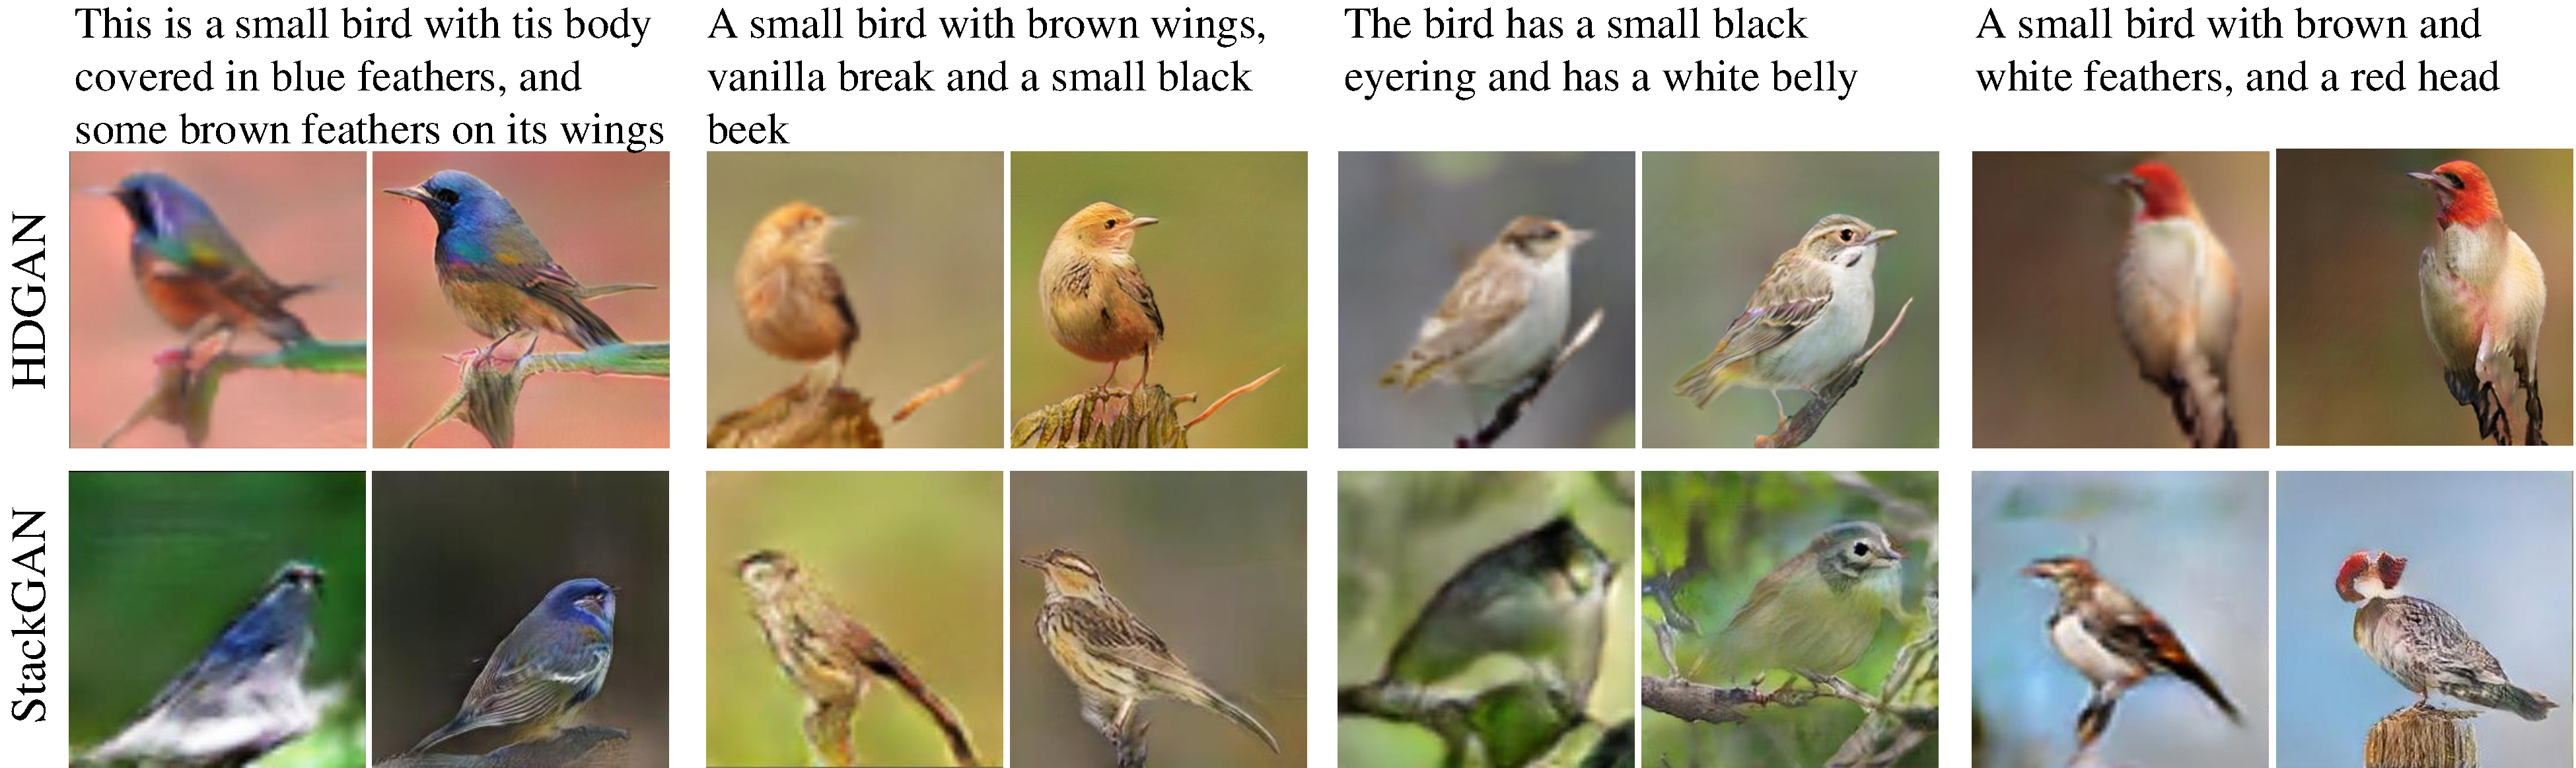
\includegraphics[width=0.99\textwidth]{figure/cub.pdf}
	\vspace{-.2cm}
	\caption{The generated images on CUB compared with StackGAN. Each sample shows the input text and generated $64^2$ (left) and $256^2$ (right) images. Our results have significantly higher quality and preserve more semantic details, for example, ``the brown and white feathers and read head'' in the last column is much better reflected in our images. Moreover, we observed our birds have more diverse poses (e.g. the frontal view in the the second and the back view forth columns).}
	\vspace{-0.2cm}
	\label{fig:vis-cub}
\end{figure*}
\begin{figure*}[t]
	\centering
	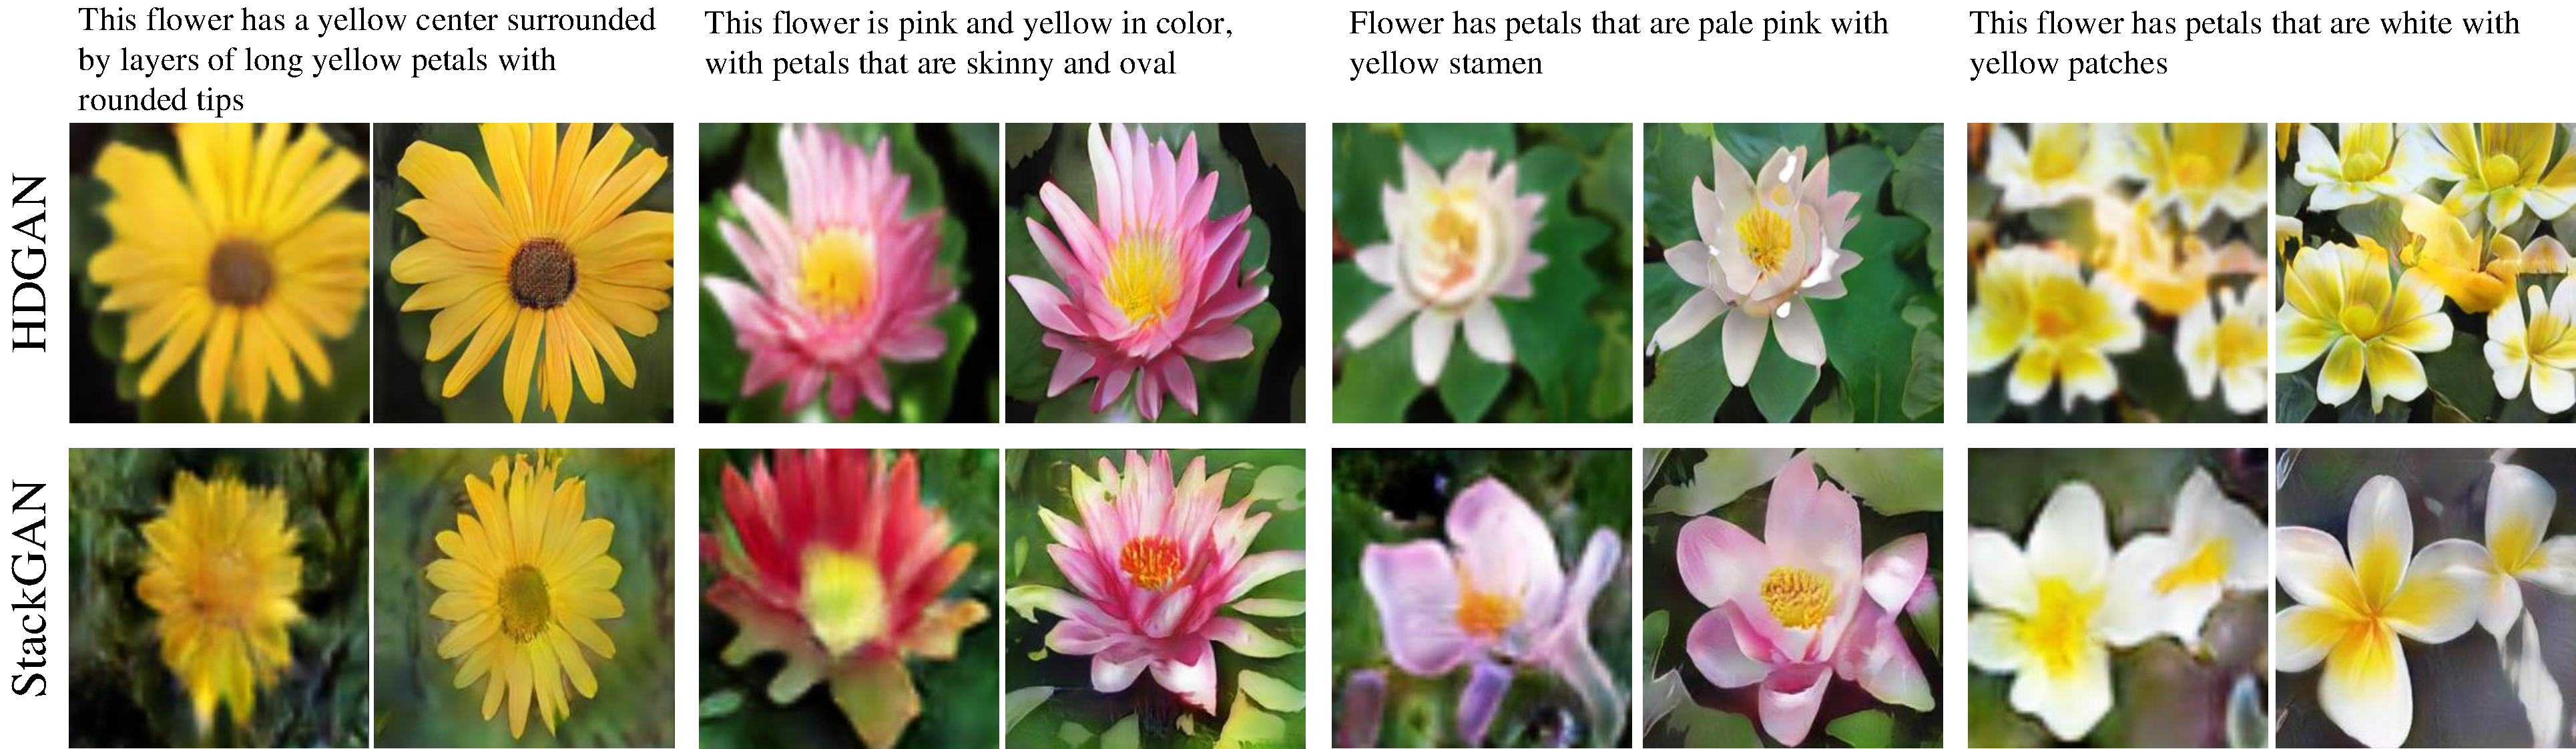
\includegraphics[width=0.99\textwidth]{figure/flowers.pdf}
	\vspace{-.2cm}
	\caption{The generated images on Oxford-102 compared with StackGAN. Our generated images perform more natural satisfiability and higher contrast and can generate complex flower structures (e.g. spiked petals) like the third example.} \label{fig:vis-oxford}
	\vspace{-.2cm}
\end{figure*}

\begin{table}[t] % retrieval
	\small
	\begin{center}
		\begin{tabularx}{.475\textwidth}{c|ccc}
			\specialrule{1.5pt}{0pt}{0pt}  
			\multirow{2}{*}{Method}	& \multicolumn{3}{c}{Dataset}	\\ \cline{2-4}
			&	 CUB		&	Oxford  & COCO		     \\ \hline
			Ground Truth	&	${.302{\pm}.151}$	&	$ {.336{\pm}.138}$			& $.426{\pm}.157$  \\ \hline
			StackGAN     &	$.228{\pm}.162$	&	 $.278{\pm}.134$			&  -		\\ 
			HDGAN 		&	$\bm{.246{\pm}.157}$	&	$ \bm{.296{\pm}.131}$ & $\bm{.178{\pm}.181}$  \\ \hline
		\end{tabularx} 
	\end{center}
	\vspace{-.4cm}
	\caption{The VS similarity evaluation on the three datasets. The higher score represents higher semantic consistency between the generated images and the text information. } \label{table:vss}
\end{table}

\subsection{Comparative Results}
To validate our method, we compare our results with GAN-INT-CLS \cite{reed2016generative}, GAWWN \cite{reed2016learning}, TAC-GAN \cite{dash2017tac}, StackGAN \cite{han2017stackgan} and also its improved version StackGAN++ \cite{han2017stackganv2}, and Progressive GAN \cite{Karras2017progressive}\footnote{StackGAN++ and Prog.GAN are two very recently released preprints we noticed. We acknowledge them as they also target at generating high-resolution images. }. We especially compare with the current state of the art, StackGAN (results are obtained from its provided models).

% Similarly with our HDGAN, it now can train $64{-}256$ directly. Each generator still take images from the bottom generator and supervised by a discriminator. Differently, our network is more like a simple Vanilla network (or a pure inverse ImageNet CNN).}. 

%StackGAN \cite{han2017stackgan} generates synthetic images up to $256{\times}256$ resolution. We show that our method can generates images up to $512{\times}512$.

Table \ref{table:score} shows the quantitative inception-score evaluation. We follow StackGAN' experiment setting to sample ${~}30,000$ $256^2$ images for evaluation.
HDGAN achieves significantly improvement compared against other methods. For example, it improves StackGAN by $.45$ and StackGAN++ by $.31$ on CUB.
HDGAN achieves competitive results with TAC-GAN on Oxford-102. TAC-GAN uses image labels to increase the discriminability of generators, while we do not use any extra knowledge. Figure \ref{fig:vis-cub} and Figure \ref{fig:vis-oxford} show the results compared with StackGAN and strongly demonstrate the superiority of HDGAN. Mover, we also qualitatively test the diversity of samples conditioned on the same text in Figure \ref{fig:multiple-test} left. It also demonstrates how well the model learned to cover the input distribution. HDGAN shows obvious more successful samples than StackGAN.

Table \ref{table:vss} shows the qualitative vs-similarity comparison results on three datasets. We also add the evaluation results on the ground truth image and sentence pair for reference. Our proposed method achieves much better results on both CUB and Oxford-102 datasets. Since we do not have a pre-trained  StackGAN model for coco dataset, we omit the comparison. This results demonstrate that HDGAN is better at capturing visual semantic correlation.

%\begin{figure}[t]
%	\centering
%	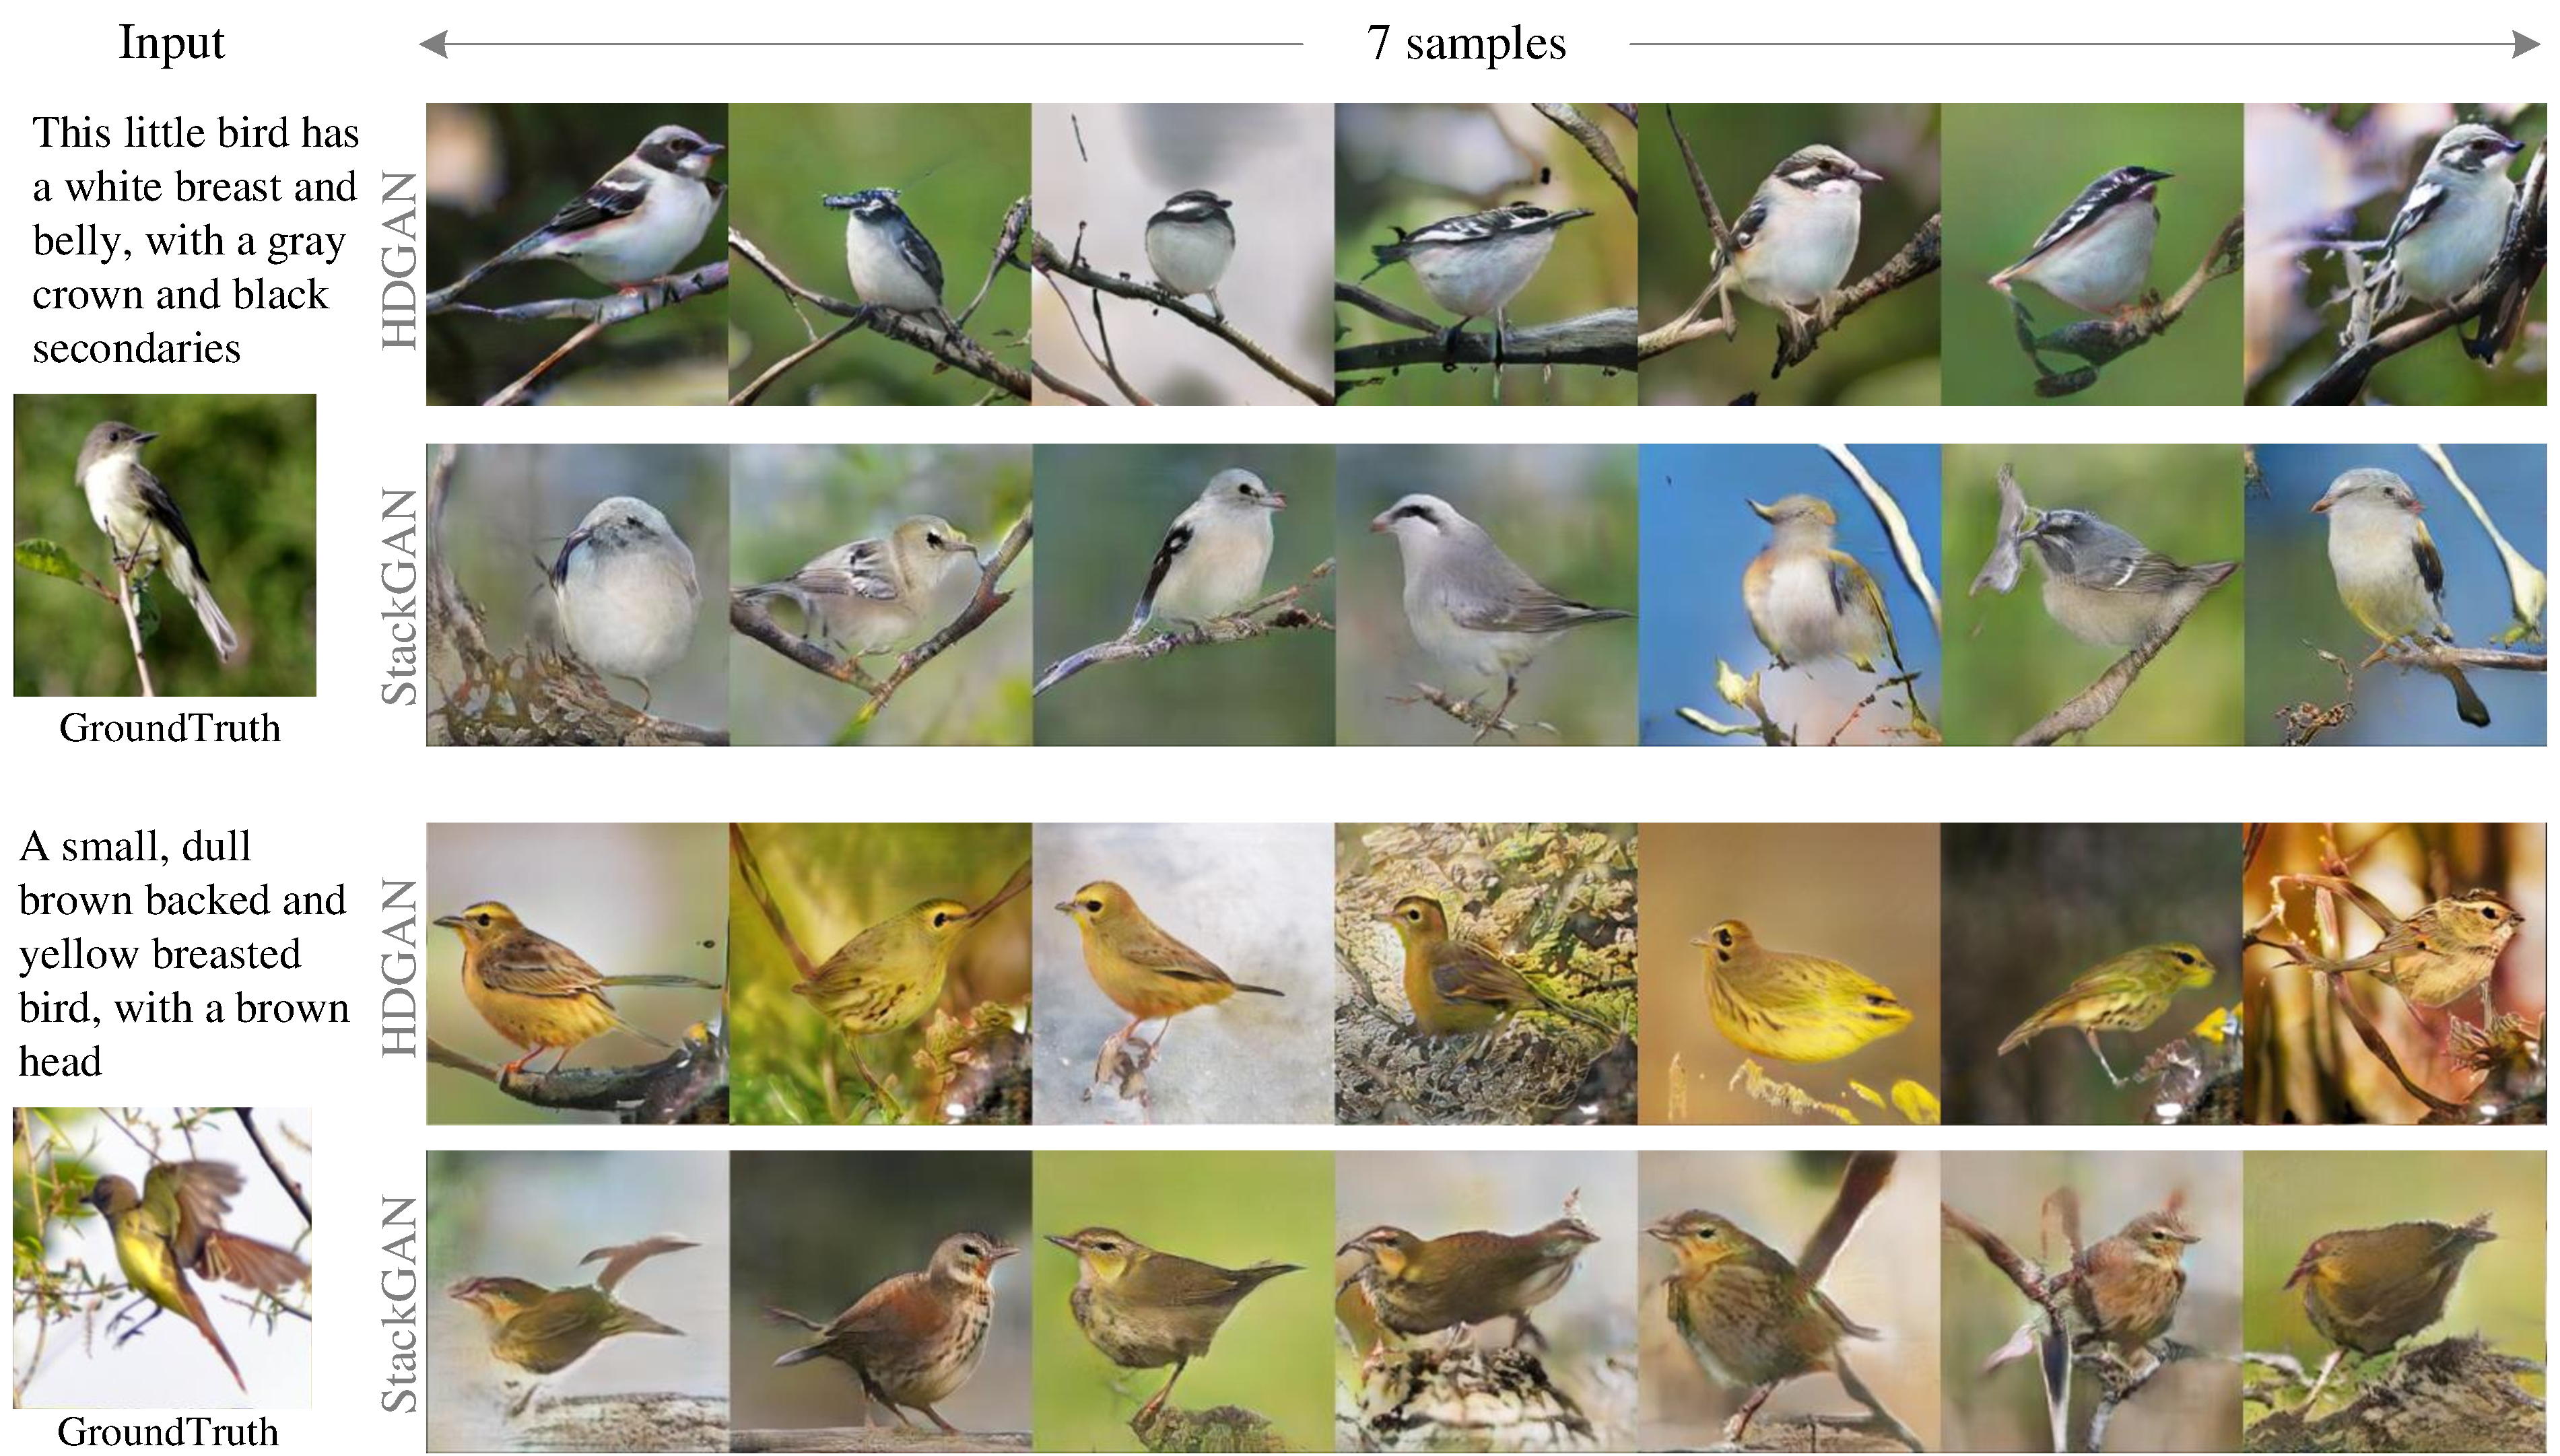
\includegraphics[width=0.499\textwidth]{figure/multisample_cub.pdf}
%	\caption{Results on Oxford} \label{fig:multires-cub}
%\end{figure}

\begin{figure*}[t]
	%	\begin{center}
	\centering
	\begin{subfigure}[t]{0.69\textwidth}
		%	\centering
		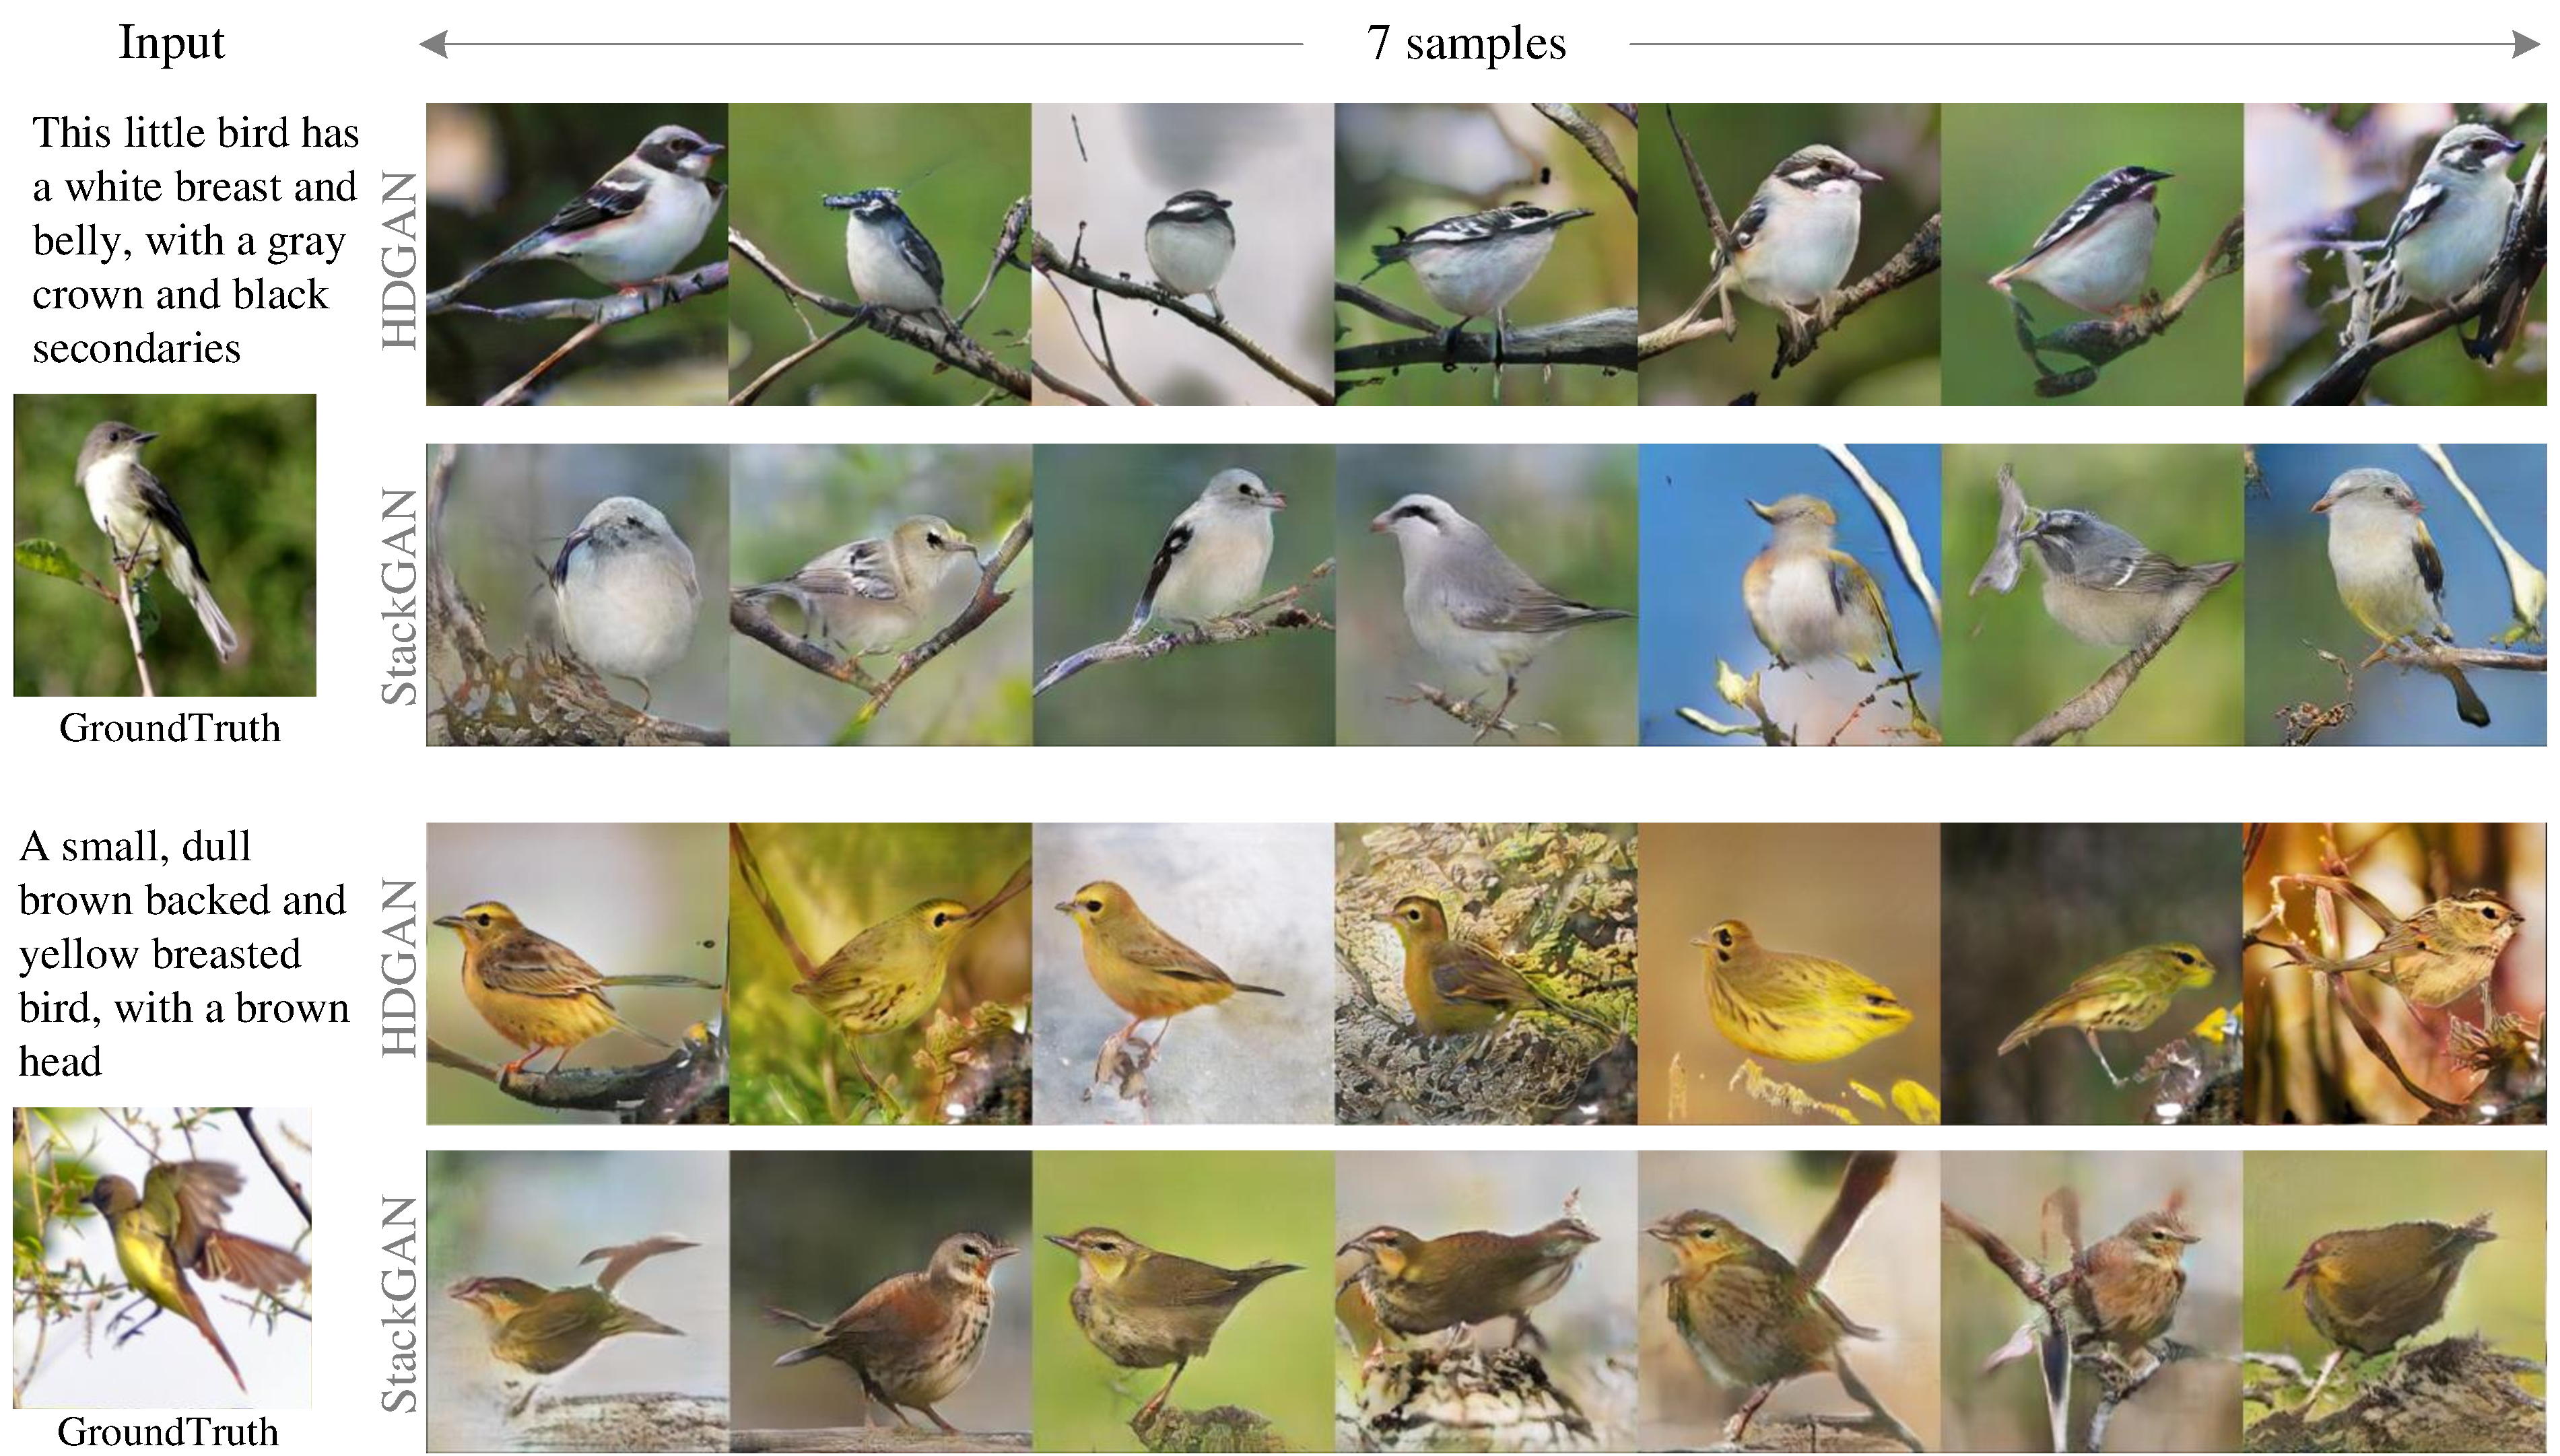
\includegraphics[width=0.99\textwidth]{figure/multisample_cub.pdf}
	\end{subfigure} 
	\begin{subfigure}[t]{0.3\textwidth}
		%	\centering
		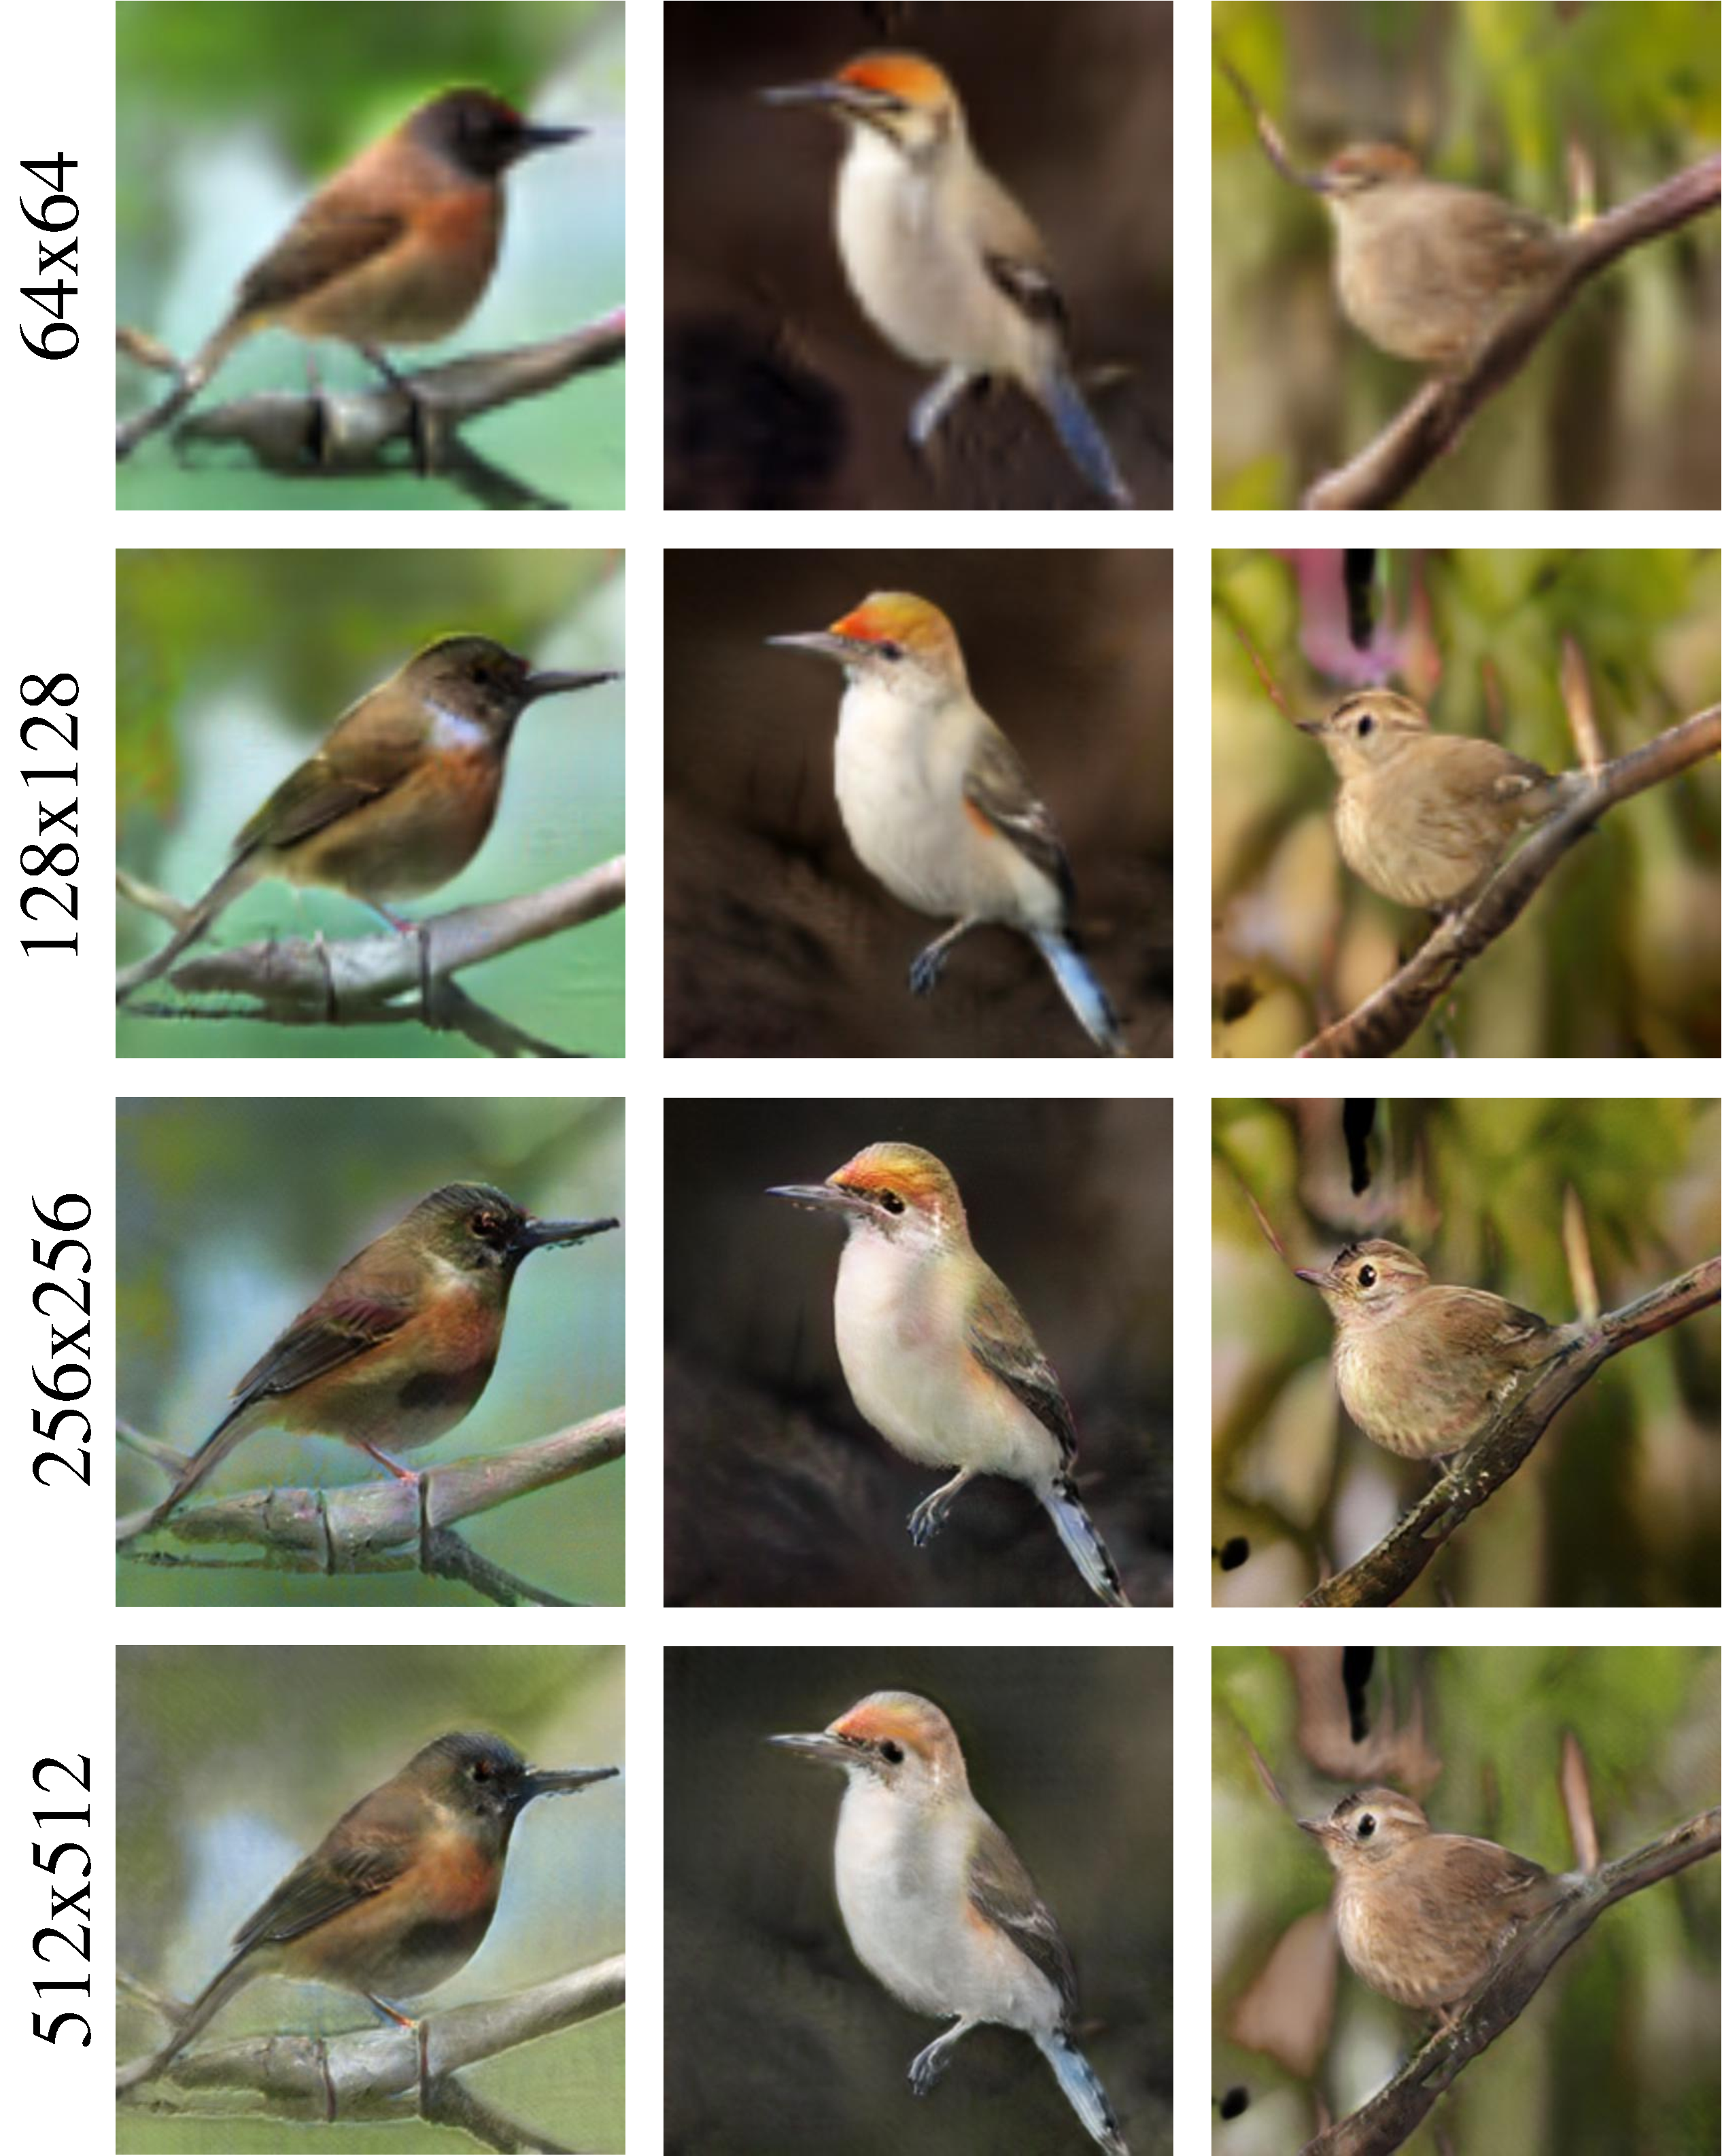
\includegraphics[width=0.99\textwidth]{figure/cub_multires.pdf}
	\end{subfigure}
	\vspace{-.2cm}
	\caption{Left: Diversity test given a single input text. The proposed HDGAN (top) show obviously more details and higher diversity. Right: Side outputs of HDGAN with increasing resolutions. Different resolutions are semantically consistent and semantic details emerges as resolution increases.  \label{fig:multiple-test}} 	\vspace{-.3cm}
	%\end{center}
\end{figure*}


\begin{table}[t] % retrieval
	\begin{minipage}[b]{0.50\linewidth}
		%\centering
		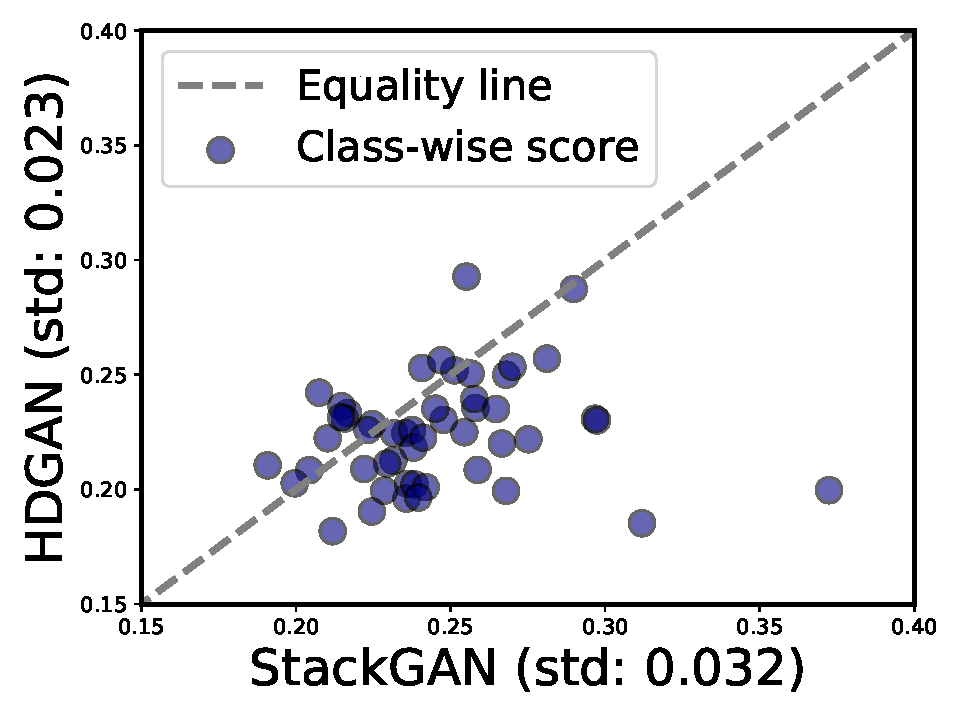
\includegraphics[width=0.99\textwidth,height=0.7\textwidth]{figure/ms_ssmi.pdf}
		\vspace{-1.8cm}
	\end{minipage} %\hfill
	\begin{minipage}[b]{0.49\linewidth}
		\begin{tabularx}{.9\textwidth}{c|c}
			\specialrule{1.5pt}{0pt}{0pt}  
			Method   &  MS-SSMI \\ \hline
			StackGAN &   0.234   \\ 
			Prog.GAN &   0.225    \\ \hline
			HDGAN    &   \textbf{0.215}    \\ \hline
		\end{tabularx}
	\end{minipage}
	\vspace{0.2cm}
	\caption{Left: Class-wise MS-SSMI evaluation. Lower score indicates higher intraclass dissimilarity. The points below the equality line represent classes our HDGAN wins. The inter-class std is shown in axis titles. Right: Overall (no class-wise)  MS-SSMI evaluation.} \label{fig:msssmi}
	\vspace{-0.4cm}
\end{table}

Table \ref{fig:msssmi} compares the MS-SSMI image quality evaluation score with StackGAN and Prog.GAN for bird image generation. StackGAN and our HDGAN use the semantic text as input so the generated images are separable in class. We randomly sample ${~}20,000$ image pairs (400 per class) and show the class-wise score in the left figure. HDGAN outperforms StackGAN in majority of classes and also has lower inter-class standard deviation ($.023$ vs. $.032$).
Prog.GAN uses noise input rather than text. We can compare with it for general measure of synthesis diversity. Following the procedure of Prog.GAN, we randomly sample ${~}10,000$ image pairs from all generated samples (We use $256^2$ images provided by the Prog.GAN online) and show the results in Table \ref{fig:msssmi} right. Our HDGAN outperforms both methods. 


\begingroup
\setlength{\intextsep}{-4pt}%
\setlength{\columnsep}{0pt}%
\begin{wrapfigure}{r}{0.24\textwidth}
	\centering
	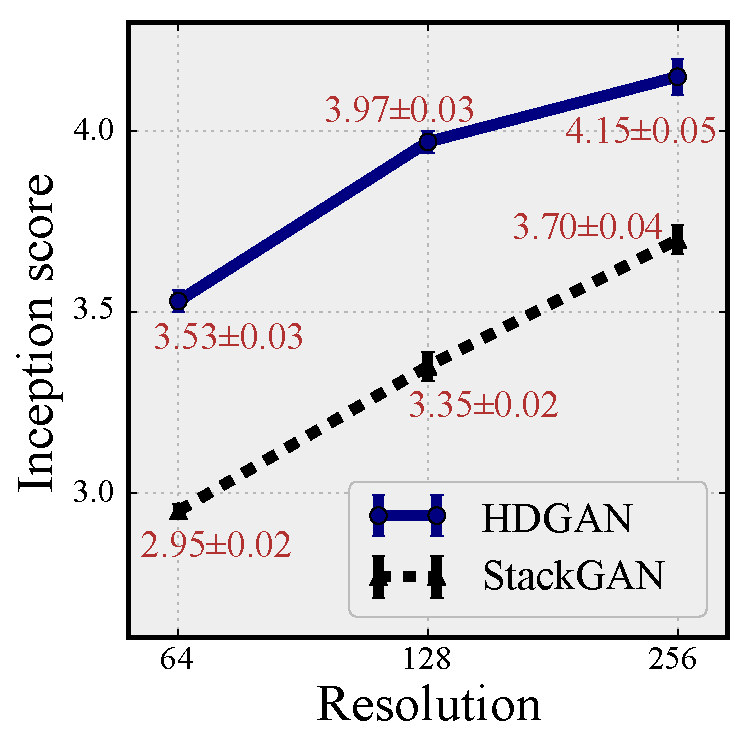
\includegraphics[width=0.245\textwidth]{figure/multiscale_inception_2.pdf}
	\vspace{-12pt}
\end{wrapfigure}
%Table \ref{table:multiscales}
The right figure compares the the multi-resolution inception score on CUB. Our results are from the side outputs of a single model. As can be observed, our $64^2$ images outperforms $128^2$ images of StackGAN and our $128^2$ images outperforms $256^2$ images of StackGAN substantially. It strongly demonstrates our HDGAN better preserves semantically consistent information in all resolutions. Figure \ref{fig:multiple-test}  right qualitatively validate this property. However, in StackGAN, the low resolution and high resolution image sometimes are visually inconsistent (see examples in Figure \ref{fig:vis-cub} and Figure \ref{fig:vis-oxford}).


\subsection{Style Transfer Using Sentence Interpolation}
Ideally, a well trained model should learn a smooth linear latent manifold of the images. To demonstrate the generalization capability of HDGAN, we generate images using the linearly interpolated embeddings between two source sentences. %%We fix the random noise input to make the object and background consistent. 
As is shown in Figure~\ref{fig:interp}, the generated images show smooth style transformation and well reflect the semantic details in sentences. 
In the first row, the generated birds gradually turn the color from yellow to brown. In the second row, more complicated sentences containing more detailed appearance information (e.g., blue peaks and yellow wing) are used, we can see that our model is still be able to successfully capture these subtle information and tune the bird appearance gradually. 




%\subsubsection{What role does noise play}
%In our model, there are two kinds of randomness injected to the input of the Generator, ie, epsilon $\epsilon$ and Gaussian noise vector $z$. 
%In this experiment, we fix the sentence embedding and one noise, and change the other random variable. For each random noise, we generate 4 different values. So In total 16 images are generated using all noise combinations, the resulting images are shown in Figure~\ref{}, $\epsilon$ and $z$ corresponds to row and column dimension, respectively. As is shown in the image, we can see that, $\epsilon$ can change the pose of the image, while $z$ is mainly responsible for the background variations. This clearly demonstrate that, our model learns to disentangle the semantic information from the pose and background information.


\subsection{On the effects of Individual Components}
\subsubsection{Hierarchically-nested adversarial training}
Our hierarchically-nested adversarial discriminators a role of regularizing the layer representations (at scale $\{64, 128, 256\}$). 
%Our full method applies it on feature maps at $\{64, 128, 256\}$. 
In Table \ref{tab:ablation} right, we compare the results by removing part of discriminators. 
As can be seen, increasing the usage of discriminators at different scales have positive effectives. And using discriminators on $64^2$ is critical (by comparing 64-256 and 128-256 cases). For now, we are unsure if adding more discriminators and adding on lower resolution would be helpful. Further investigation will be conducted to validate it.
StackGAN emphasizes the importance of using text embeddings with mid-level features of the $256^2$ generator by showing an large drop from $3.7$ to $3.45$ without doing so, which helps maintains the diversity and semantic consistency. While in our method, we only use text embeddings at the input. Our significantly improved results demonstrate that effectiveness of the hierarchically-nested adversarial training to achieve this goal. 

\subsubsection{On the Local Image Loss}

\textcolor{red}{We also study the effectiveness of the proposed local image loss. We conduct experiments with using architecture with side output 64$\times$64, 128$\times$128 and 256 $\times$ 256 using CUB dataset. 
As can be seen in Table\ref{tab:local_loss}, we can see that by removing local image loss (denoted as "No Local"), the inception score drop from \textcolor{red}{4.27} to \textcolor{red}{3.8}. To quantitatively compare the results, we also show generated results using two model in Figure \ref{local_or_not}, We can see that, although both models can successfully capture the semantic correspondence between image and sentence, 256$\times$ 256 results generated by model trained with local image loss provide more local fine-grained details, thus improving the visual quality. }

\begin{figure}[t]
	\centering
	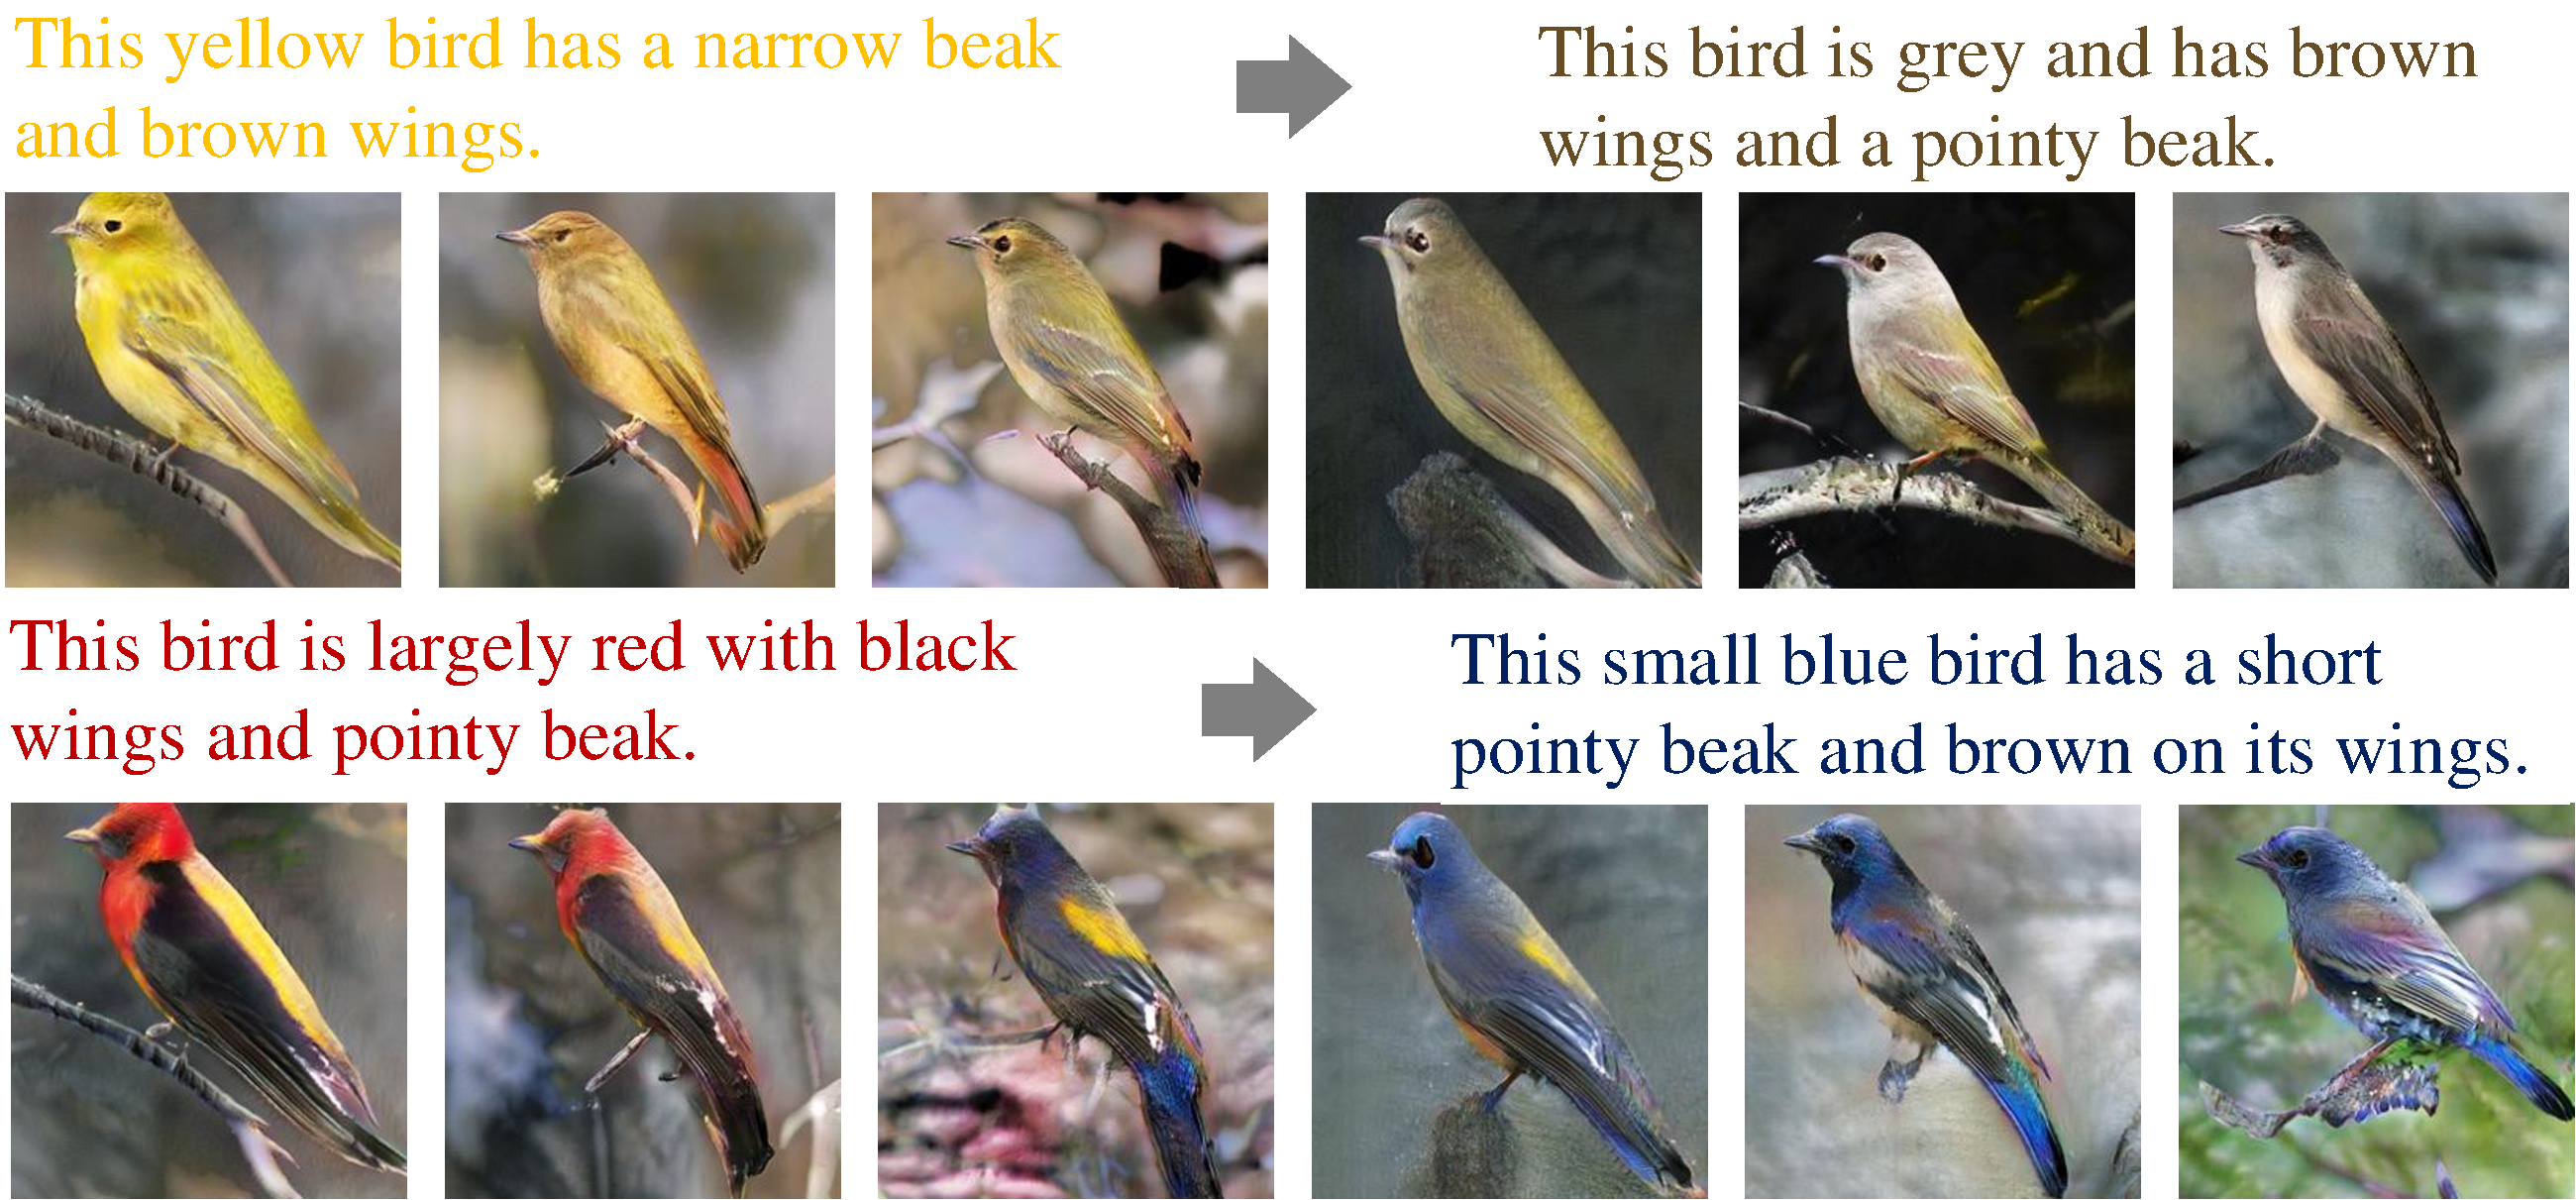
\includegraphics[width=0.48\textwidth]{figure/interp.pdf}
	\vspace{-.5cm}
	\caption{Text embedding interpolation from the source to target sentence results in smooth image style changes to match the targeting sentence. } \label{fig:interp}
	\vspace{-.3cm}
\end{figure}

%\begin{table}[t] % retrieval
%	\begin{center}
%		\begin{tabularx}{.268\textwidth}{ccc|c}
%			\specialrule{1.5pt}{0pt}{0pt}  
%			\multicolumn{3}{c|}{Components}	&  \multirow{2}{*}{Score}	\\ \cline{1-3}
%			64	& 128	& 256 			& 		\\ \hline
%			&  		&	\checkmark	&	${3.52{\pm}.04}$	\\ 
%			&  	\checkmark	&	\checkmark	&	${3.99{\pm}.04}$	\\
%			\checkmark	&  			&	\checkmark	&  ${4.14{\pm}.03}$		\\
%			\checkmark	&  \checkmark		&	\checkmark	&	${4.15{\pm}.05}$ \\
%			
%		\end{tabularx}
%	\end{center} \vspace{-.4cm}
%	\caption{Ablation study for hierarchically-nested adversarial supervision.} \label{table:deep-nest}
%\end{table}

%\begin{table}[t] % retrieval
%	\label{tab:local_loss}
%	\begin{center}
%		\begin{tabularx}{.43\textwidth}{c|ccc}
%			\specialrule{1.1pt}{0pt}{0pt}  
%			Metric 			 		&   wo/Img 	 & w/global     &   w/local	\\  \hline
%			MS-SSMI                 &   $-$      &   $-$           &	$.215$ \\  \hline
%			VS similarity           &   $-$      &   $-$           &	$.246{\pm}.157$ \\ \hline
%			Inception score         &   $-$ 	 &   $-$		   &    $4.15{\pm}.05$ \\
%		\end{tabularx}
%	\end{center} \vspace{-.4cm}
%	\caption{Results using three quantitative evaluation metrics on birds dataset.} \label{table:imgloss}
%\end{table}

\begin{table}[t] % retrieval
	\small
	\begin{minipage}[b]{0.5\linewidth}
			\begin{tabularx}{.98\textwidth}{c@{\hskip1pt}|c@{\hskip1pt}c@{\hskip1pt}}
				\specialrule{1.5pt}{0pt}{0pt}  
				Metric 			&   VS 	 & MS-SSMI   	\\  \hline
				w/o Img         &   $.25{\pm}.16$      &   $.215$           \\  \hline
				w/ global       &   $-$      &   $-$           \\ \hline
				w/local         &   $-$ 	 &   $-$		    \\ \hline
			\end{tabularx}
		\vspace{-0.8cm}
	\end{minipage} %\hfill
	\begin{minipage}[b]{0.49\linewidth}
		\begin{tabularx}{.98\textwidth}{ccc|c}
			\specialrule{1.5pt}{0pt}{0pt}  
			\multicolumn{3}{c|}{Components}	&  \multirow{2}{*}{\thead{Inception \\ score}}	\\ \cline{1-3}
			64	& 128	& 256 			& 		\\ \hline
			&  		&	\checkmark	&	${3.52{\pm}.04}$	\\ 
			&  	\checkmark	&	\checkmark	&	${3.99{\pm}.04}$	\\
			\checkmark	&  			&	\checkmark	&  ${4.14{\pm}.03}$		\\
			\checkmark	&  \checkmark		&	\checkmark	&	${4.15{\pm}.05}$ \\ \hline
			
		\end{tabularx}
	\end{minipage}
	\vspace{-0.2cm}
	\caption{Ablation study on the local adversarial loss (left table) and hierarchically-nested adversarial learning (right table). See text for detailed explanation.} \label{tab:ablation}
\end{table}


\subsection{Design principles}
%Note that for text-to-image synthesis, StackGAN is the only successful method to generate $256{\times}256$ images.
StackGAN shows the difficulty of directly training a vanilla $256{\times}256$ GAN to generate meaningful images. 
We test this extreme case using our method by removing all nested intermediate discriminators (the first row of Table \ref{tab:ablation} left). Our method still generates fairly good results. 
%Figure \ref{fig:vallina-res} shows the qualitatively results. 
Based on our experience, the success is because of our effective generator designs that helps gradient flows.

Initially, we tried to share top layers of the hierarchical discriminators of HDGAN inspired by \cite{liu2017unsupervised} with an intuition to reduce their variances and unify their common goal (i.e. differentiates real and fake despite difficult scales). However, we did not find benefits from this mechanism and our independent discriminators can be trained very stably. 

%\textbf{Advantages}
%The advantages of our hierarchical-nested adversary are clearer from different views, compared with the popular stacking GAN strategy \cite{}. 
%First, it is memory efficient. 
%When viewing it as ensembled multi-scale GAN (Figure \ref{}), each GAN fully uses the parameters of its lower resolution GAN. Usually, a deeper generator is necessary to compact a discriminator. Since the depth of discriminator increases as image resolution increases, if stacking separate GANs based on low resolution GAN outputs, much more layers are needed in generators as wells. While in our method, for instance, from a $64^2$ GAN to a $128^2$ GAN, only a minimum two conv layers ($1$-repeat res-blocks) are needed. 
%
%Second, it fully enjoys top-down knowledge. 
%The low resolution can not use high resolution information in the stacking GAN strategy. While in our method, it is easy to see the low resolution GAN enjoys knowledge from higher resolution. As an evidence, our $64^2$ synthetic images have higher inception score than $64^2$ and even $128^2$ images of StackGAN (see Section 5).


\section{Conclusion}
In this paper, we present an effective and end-to-end method to tackle the problem of generating high-resolution images conditioned on text descriptions. We introduce a novel hierarchical-nested adversarial discriminators to regularize the mid-level representations of a generator. To improve the model's capability to render fine-grained local details, we propose a multi-purpose discriminator loss to emphasize local patch realism as well as matching aware pair. We also introduce a new evaluation metric for text-to-image synthesis to evaluate the semantic consistency between generated images and conditioned text.
Extensive experiment results demonstrate that our method, namely HDGAN, performs significantly better than existing state of the arts.


{\small
\bibliographystyle{ieee}
\bibliography{reference_zizhao,egbib}
}

\end{document}
